% !TeX document-id = {774b65cd-7beb-4446-a11b-6d182c132ee4}
% !TeX TXS-program:compile = txs:///pdflatex/[--shell-escape]
\documentclass[letterpaper,12pt]{book}
\setlength{\parindent}{0pt}
\usepackage[margin=1in]{geometry}
\usepackage[utf8]{inputenc}
\usepackage{fancyhdr}
\usepackage{graphicx}
\usepackage{tikz}
\usetikzlibrary{positioning,calc}
\usepackage{enumitem}
\usepackage{float}
\raggedbottom
\usepackage{url}
\usepackage{hyperref}
\newcommand{\appref}[1]{\hyperref[#1]{Appendix~\ref*{#1}}}
%\usepackage{showframe}
\usepackage{listings}
\usepackage{pdfpages}
\pdfminorversion=7
\setcounter{secnumdepth}{3}
\setcounter{tocdepth}{2}
\usepackage{minted}
\setminted{
    fontsize=\small,
    linenos,
    breaklines,
    breakanywhere,
    autogobble
}

\usepackage{booktabs}

\fancyhf{}
\fancyhead[LE,RO]{\thepage}
\fancyfoot[L]{\manualdate}
\fancyfoot[C]{\manualrev}
\renewcommand{\headrulewidth}{0pt}
\renewcommand{\footrulewidth}{0.4pt}
\fancypagestyle{plain}{
    \fancyhf{}
    \fancyhead[LE,RO]{\thepage}

    \fancyfoot[L]{\manualdate}
    \fancyfoot[C]{\manualrev}

    \renewcommand{\headrulewidth}{0pt}
    \renewcommand{\footrulewidth}{0.4pt}
}


\newcommand{\manualdate}{\today}
\newcommand{\manualrev}{Rev. 1}

\author{Michael Capotosto}
\title{zPSC Calibration and Test Manual}
\date{\manualdate\\[1em]
    \small \manualrev\\
}

\begin{document}

    \frontmatter
    \maketitle
    \tableofcontents

    \mainmatter
    \pagestyle{fancy}
    % !TeX root = ../main.tex

\chapter{Introduction}
\label{chap:Introduction}

    % !TeX root = ../main.tex

\chapter{Cable Assemblies and Harnesses}
\label{chap:Cable Assemblies and Harnesses}
\section{Overview}
This chapter provides a brief overview of the makeup of various cable assemblies used in the sections to follow. Some cables are off-the-shelf cables with gender changers installed on one end. Others are made up of commercial cable assemblies with fly leads that must connect to breakout boards.\\\\
Some off the shelf fiber and network patch cables will be required. 
\subsection{2-Channel DCCT Cable}
This cable consists of a Molex Micro-D15 cable, 72" long, fly lead, connecting to a Winford HD26 breakout board. 
\begin{itemize}
	\item 1x Molex 834229018 72" Micro-D15 Fly Lead Cable
	\item 1x Winford BRKEGD26HDF-T HD26F Breakout Board
\end{itemize}
\begin{figure}[H]
	
\includegraphics[width=\textwidth]{Diagrams/2Ch_DCCT_Cable}
	\caption{Pinout of 2-Channel microD15 to HD26 Cable}
\end{figure}

\subsection{4-Channel DCCT Cable}
This cable assembly consists of two parts: 
\begin{itemize}
	\item 1x Amphenol CS-DSDHD26MF0-005 1.52m HD26 M/F Cable
	\item 1x NorComp Inc. GCHDLP26F26F HD26 F/F Gender Changer
\end{itemize}

\subsection{Power Supply Channels 1 through 4 ATE Interface Cables}
This cable assembly consists of two parts:
\begin{itemize}
	\item 4x Molex 83424-9062 Micro-D25 to DB25 
	\item 4x L-com DGB25F DB25F/F Gender Changer
\end{itemize}

\subsection{SFP Transceivers}
Quantities depend on unit type and test workstation configuration. One SFP port is used for timing/event code tests on all units.\\\\
If testing FOFB, two more SFPs are required - the NSLS-II test stand uses one active copper and one fiber; though the simplest test setup would use two active copper SFPs. 
\begin{itemize}
	\item Fiber SFP: ATGBICS AFBR-57D7APZ-C or equivalent (8.5G+ SFP+, 850nm MM)
	\item Active Copper SFP: Finisar FCLF8522P2BTL or equivalent
\end{itemize}

\subsection{Other Miscellaneous Cables}
Other miscelaneous cables needed include:
\begin{itemize}
	\item CAT6 Network cables
	\item OM3 LC/LC Duplex Fiber Patch Cables (e.g. FS.com SKU 40233)
	\item IEC C13 to NEMA 5-15P Power Cords
	\item Assorted discrete wires for DC power, signal, 16-18AWG
\end{itemize}
    % !TeX root = ../main.tex
\chapter{ATE Connections}
\label{chap:ATE}
\section{Overview}
	\noindent\textbf{On initial setup,} there are a few fixed connections that need to be made to the ATE:
	\begin{itemize}[noitemsep, topsep=0pt]
		\item Current Shunt: Connect this to a resistance standard for calibrations, or to a wire loop if not being used for current measurement
		\item $\pm15V$ Supply: Connect this to a split supply, draws less than 400mA under full load
		\item Network: Connect to the local test network
		\item SD Card must be configured once, but does not require any regular changes
		\item Jumpers: Install jumpers in J8-9, J12-13,  J19-20, JJ23-24, J30-31, J34-35, J41-42, and J45-J46 for normal operations.
	\end{itemize}

	\noindent\textbf{\\\\For every device under test:}
	\begin{itemize}[noitemsep, topsep=0pt]
		\item Channel 1, 2, 3, and 4 Power Supply Cables: These cables connect to each of the micro-D Power Supply I/O connectors on the rear of the PSC
		\item Tuning Boards: Tuning boards must be installed to match the loads being tested.
		\item DCCT Cable must be connected for every PSC. There are two cables - one for 4-Channel units, and another for 2-Channel units. 
	\end{itemize}
	
	\begin{figure}[H]
		\centering
		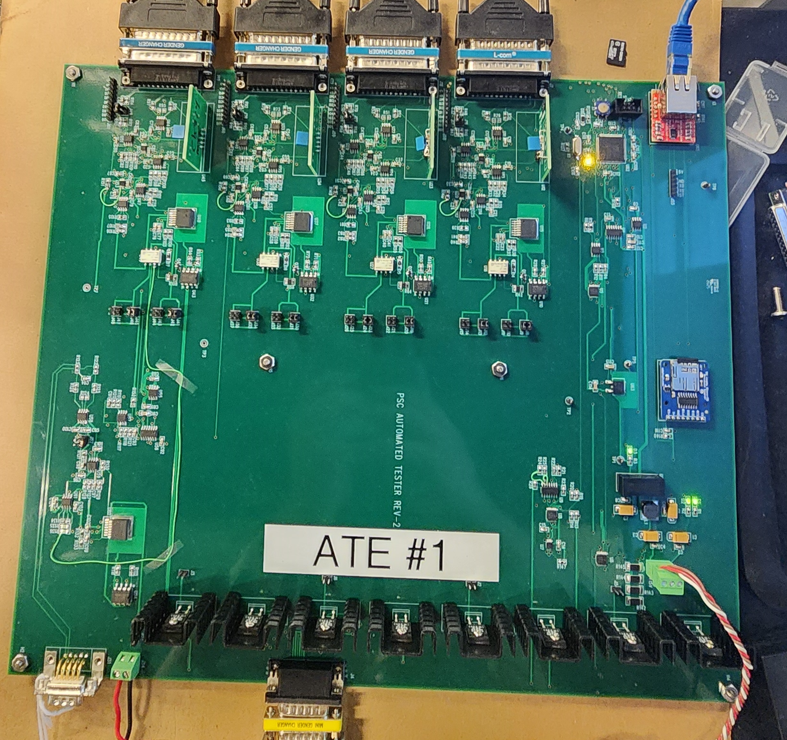
\includegraphics[width=6in]{Pictures/ATE_Cropped}
		\caption{ATE \#1}
	\end{figure}

	\subsection{ATE Test Rack at NSLS-II}
		\begin{figure}[H]
			\centering
			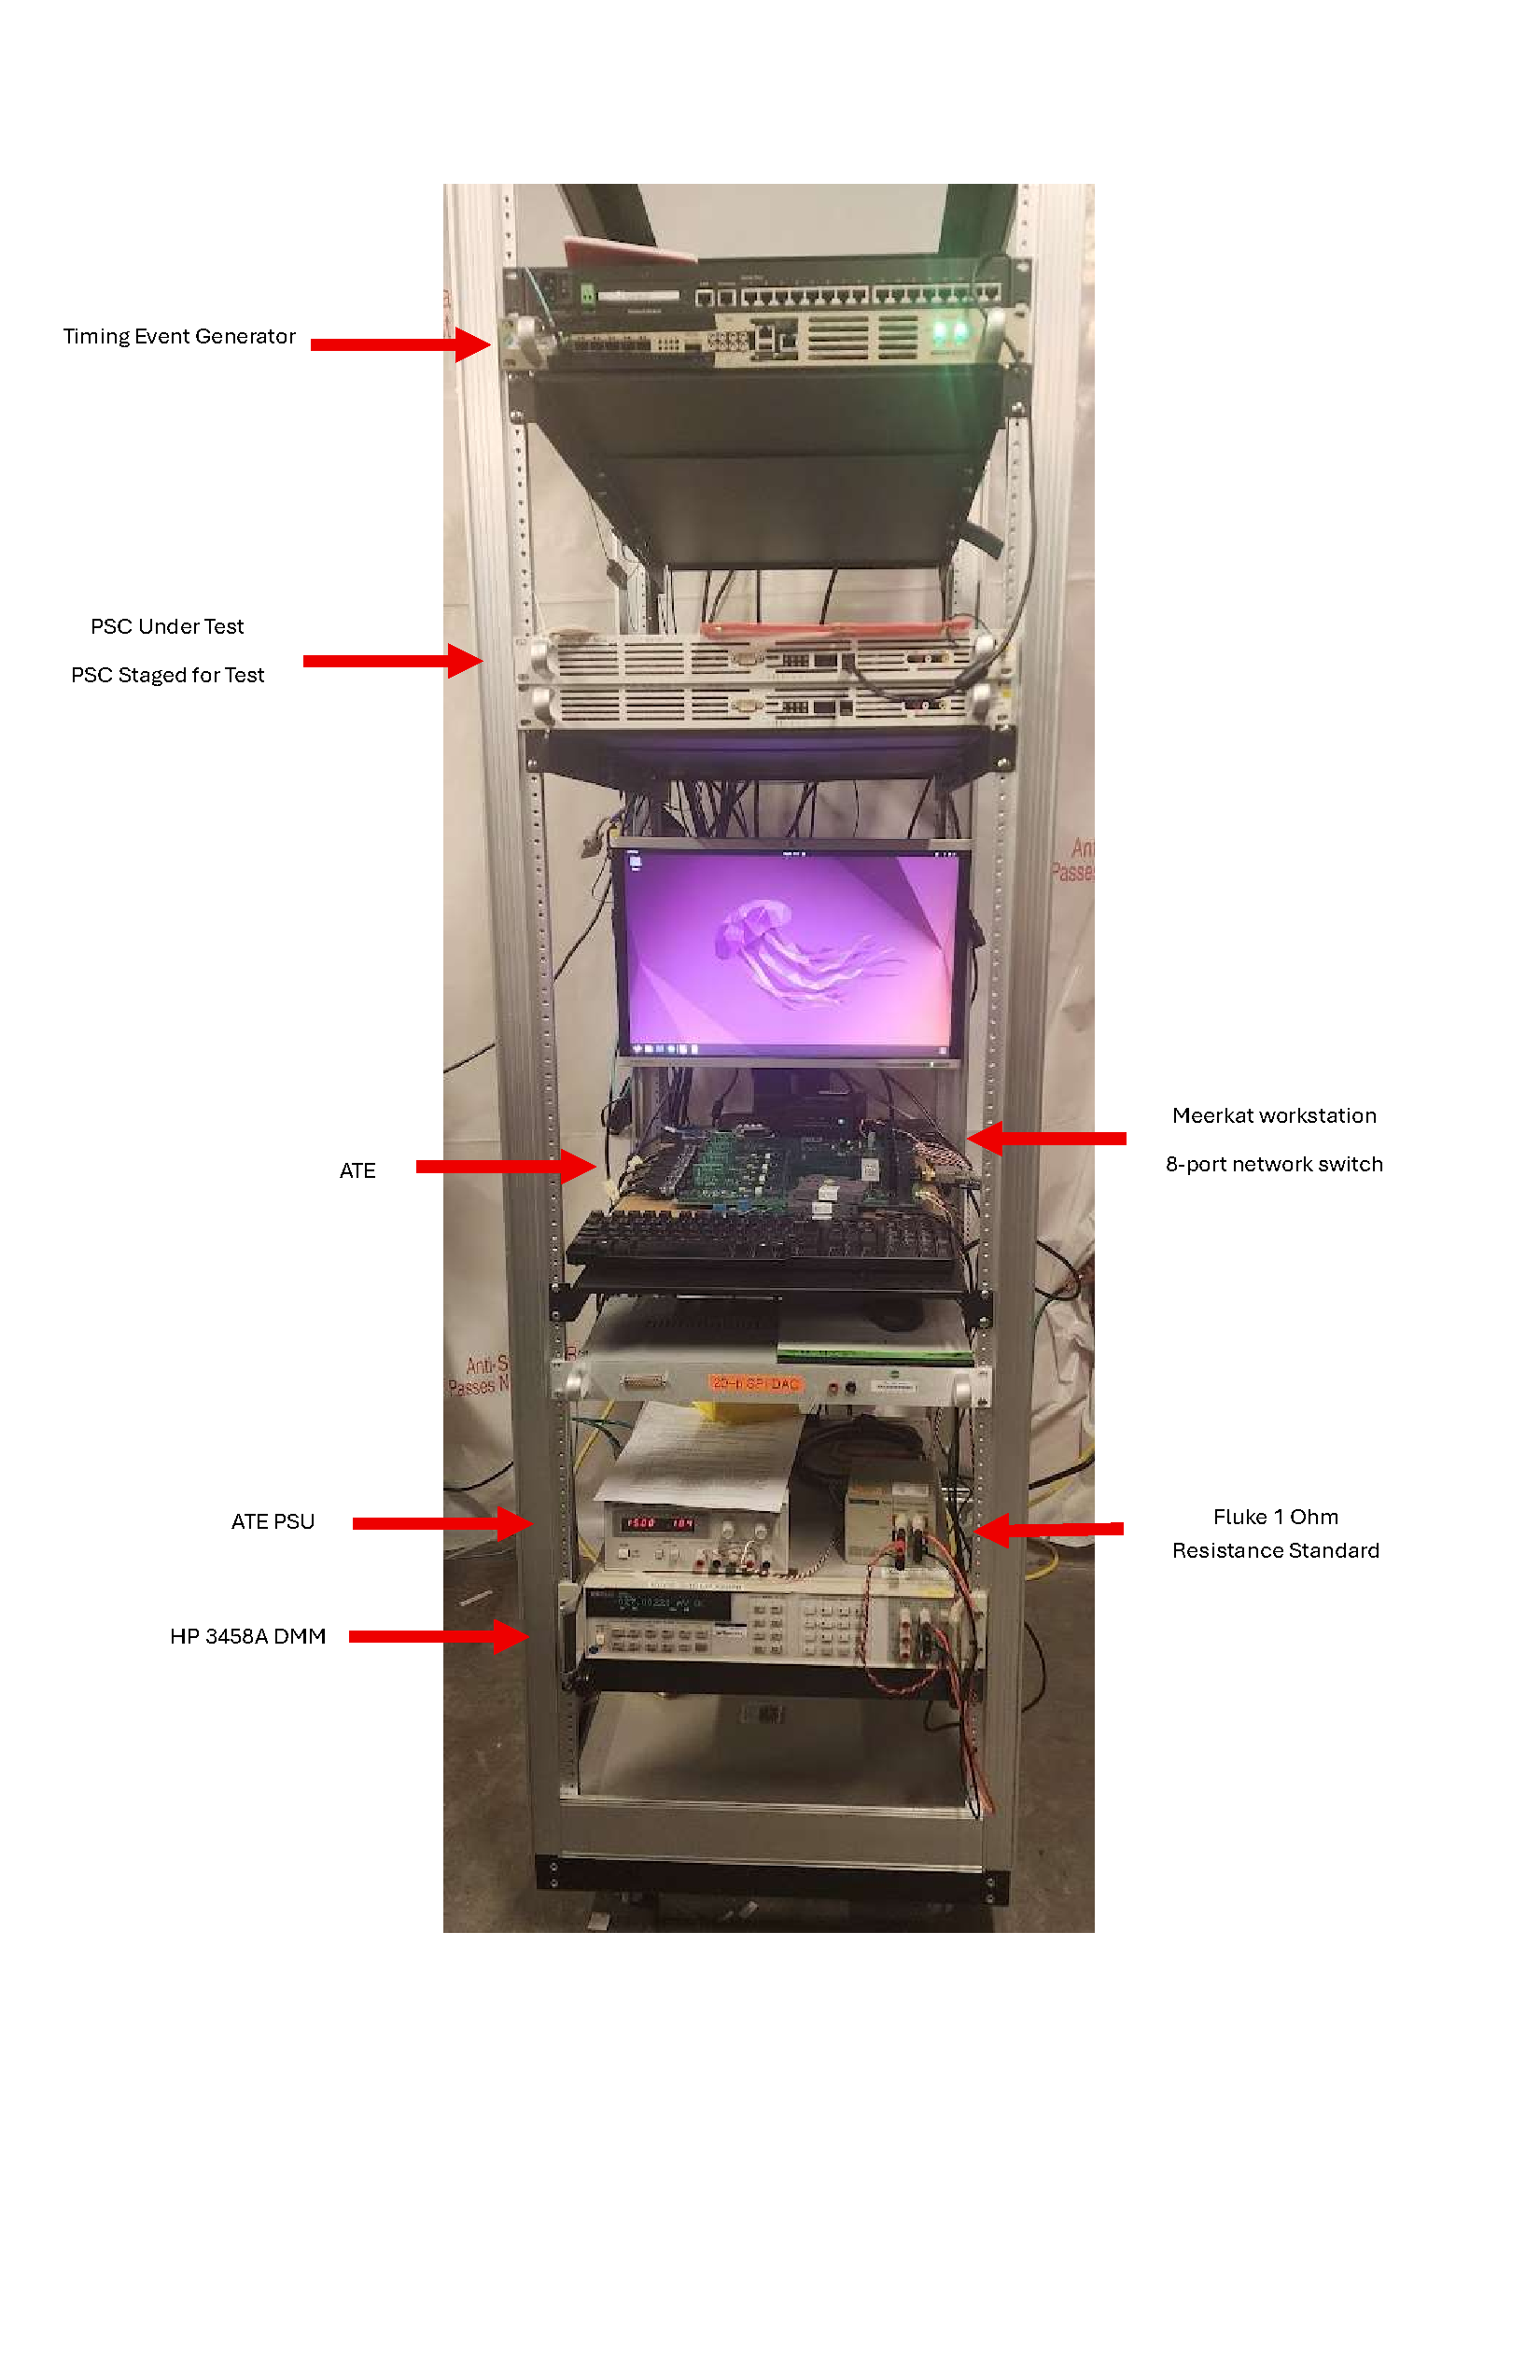
\includegraphics[
			width=5.5in,
			%height=0.85\textwidth,
			keepaspectratio
			]{Pictures/TestRackAnnotated}
		\end{figure}
		
\section{Connections}
	\begin{figure}[H]
	\centering
	\resizebox{\textwidth}{!}{%
		\begin{tikzpicture}[
			>=latex,
			chassis/.style={
				draw,
				rectangle,
				line width=0.8pt,
				align=center
			},
			module/.style={
				draw,
				rectangle,
				minimum width=2.5cm,
				minimum height=0.75cm,
				align=center,
				font=\small
			},
			block/.style={
				draw,
				rectangle,
				minimum width=3.0cm,
				minimum height=1.0cm,
				align=center,
				font=\small
			},
			shuntblock/.style={
				draw,
				rectangle,
				minimum width=4cm,
				minimum height=1.4cm,
				align=center,
				font=\small
			}
			]
			
			% ==================================================
			% PSC CHASSIS
			% ==================================================
			\node[
			chassis,
			minimum width=3.4cm,
			minimum height=6.6cm
			] (psc) at (0,0) {};
			
			\node[font=\Large\bfseries] at (0,2.75) {PSC};
			
			\node[module] (dcct) at (0,1.7) {DCCT};
			\node[module] (ch1)  at (0,0.7) {CH1};
			\node[module] (ch2)  at (0,-0.3) {CH2};
			\node[module] (ch3)  at (0,-1.3) {CH3};
			\node[module] (ch4)  at (0,-2.3) {CH4};
			
			% ==================================================
			% ATE CHASSIS
			% ==================================================
			\node[
			chassis,
			minimum width=3.8cm,
			minimum height=13.5cm
			] (ate) at (6.0,-2.5) {};
			
			\node[font=\Large\bfseries] at (6.0,3.4) {ATE};
			
			\node[module] (ate_dcct) at (6.0,1.7) {DCCT};
			\node[module] (ate_ch1)  at (6.0,0.7) {CH1};
			\node[module] (ate_ch2)  at (6.0,-0.3) {CH2};
			\node[module] (ate_ch3)  at (6.0,-1.3) {CH3};
			\node[module] (ate_ch4)  at (6.0,-2.3) {CH4};
			
			\node[module] (ate_pwr) at (6.0,-4.0) {$\pm15$ V};
			\node[module] (ate_net) at (6.0,-5.4) {Network};
			
			% ATE Current Shunt block inside chassis
			\node[
			shuntblock,
			minimum width=3.2cm,
			minimum height=1.8cm
			] (ate_shunt) at (6.0,-7.4)
			{
				ATE Current Shunt\\
				Terminal Block
			};
			
			% ==================================================
			% PSC -> ATE CONNECTIONS
			% ==================================================
			\draw[->] (dcct.east) -- (ate_dcct.west);
			\draw[->] (ch1.east)  -- (ate_ch1.west);
			\draw[->] (ch2.east)  -- (ate_ch2.west);
			\draw[->] (ch3.east)  -- (ate_ch3.west);
			\draw[->] (ch4.east)  -- (ate_ch4.west);
			
			% ==================================================
			% POWER SUPPLY + NETWORK SWITCH
			% ==================================================
			\node[block] (supply) at (0,-4.0)
			{
				$\pm15$ V\\
				Power Supply
			};
			
			\node[block] (switch) at (0,-5.4)
			{
				Network\\
				Switch
			};
			
			\draw[->] (supply.east) -- (ate_pwr.west);
			\draw[->] (switch.east) -- (ate_net.west);
			
			% ==================================================
			% RESISTANCE STANDARD
			% ==================================================
			\node[
			block,
			minimum width=6cm,
			minimum height=4cm,
			inner sep=12pt
			] (resistor) at (14.0,-7.4)
			{
				4-Terminal\\[6pt]
				Resistance Standard\\[6pt]
				\quad Fluke 742A-1 or equivalent\quad\mbox{}\\[6pt]
				1 Ohm
			};
			
			% ==================================================
			% DMM
			% ==================================================
			\node[
			block,
			minimum width=6cm,
			minimum height=3.6cm
			] (dmm) at (22.0,-7.4)
			{
				DMM\\[10pt]
				HP 3458A or equivalent
			};
			
			% GPIB block INSIDE DMM
			\node[
			draw,
			rectangle,
			minimum width=3.2cm,
			minimum height=0.8cm,
			font=\small
			] (gpib) at ($(dmm.south)+(0,0.4)$)
			{GPIB};
			
			% ==================================================
			% PROLOGIX
			% ==================================================
			\node[
			draw,
			rectangle,
			minimum width=5cm,
			minimum height=1.2cm,
			font=\small
			] (prologix) at ($(dmm.south)+(0,-2.0)$)
			{Prologix GPIB Adapter};
			
			\draw[->, thick] (gpib.south) -- (prologix.north);
			
			% ==================================================
			% SIDE LABELS
			% ==================================================
			\node[
			draw,
			rotate=90,
			fill=white,
			inner sep=4pt
			]
			at ($(resistor.west)+(0.3,0)$)
			{CURRENT};
			
			\node[
			draw,
			rotate=90,
			fill=white,
			inner sep=4pt
			]
			at ($(resistor.east)+(-0.3,0)$)
			{SENSE};
			
			\node[
			draw,
			rotate=90,
			fill=white,
			inner sep=4pt
			]
			at ($(dmm.west)+(0.35,0)$)
			{Input};
			
			% ==================================================
			% MEASUREMENT CHAIN CONNECTIONS
			% ==================================================
			\draw[->, thick] (ate_shunt.east) -- (resistor.west);
			\draw[->, thick] (resistor.east) -- (dmm.west);
			
		\end{tikzpicture}%
	}
	\caption{ATE Connection Block Diagram}
	\label{fig:psc_ate_block_diagram}
\end{figure}

\begin{figure}[H]
	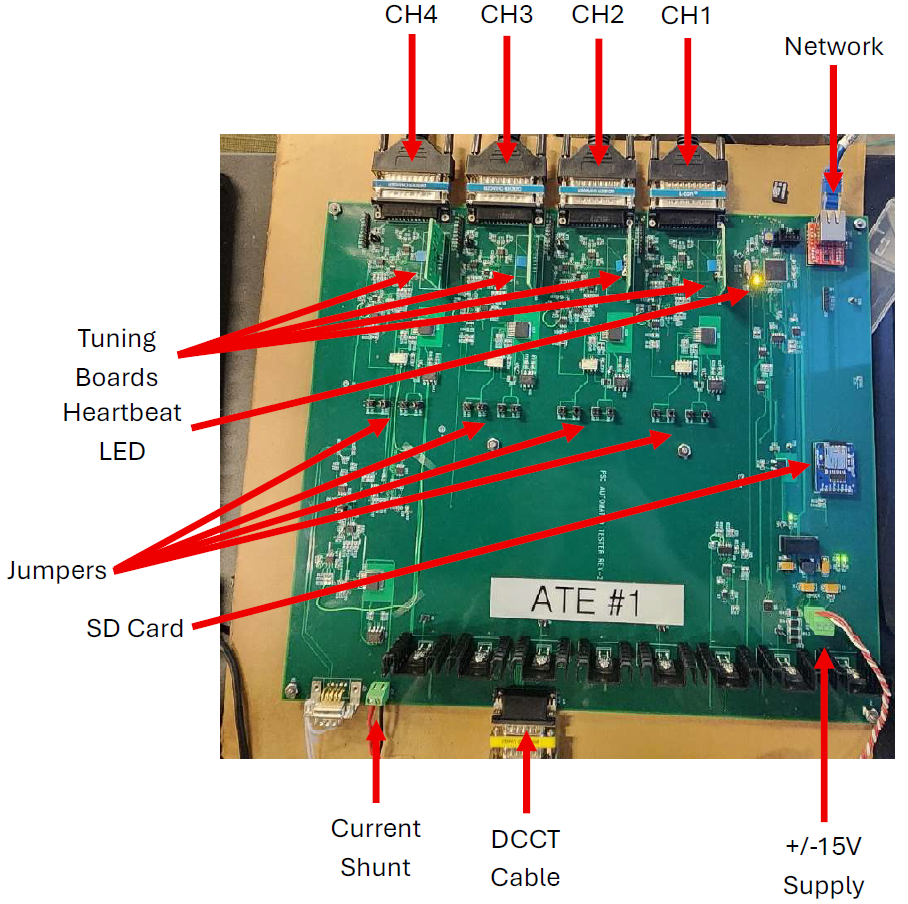
\includegraphics[width=\textwidth]{Pictures/ATE_Annotated}
	\caption{Annotated ATE Board}
\end{figure}

\newpage
\subsection{Current Measurement Loop/DMM Connection}
The DMM is connected to the workstation via a GPIB adapter from Prologix. These are available in both USB and Ethernet forms.\\\\
%
\begin{center}
	\setlength{\fboxrule}{1.5pt}
	\setlength{\fboxsep}{6pt}
	\fbox{
		\parbox{0.9\textwidth}{
			\textbf{If the DMM/Resistance standard is not used, a jumper must be connected across this terminal block on the ATE if CALDAC is to be used!}
		}
	}
\end{center}

\begin{figure}[H]
	\centering
		\resizebox{0.75\textwidth}{!}{%
		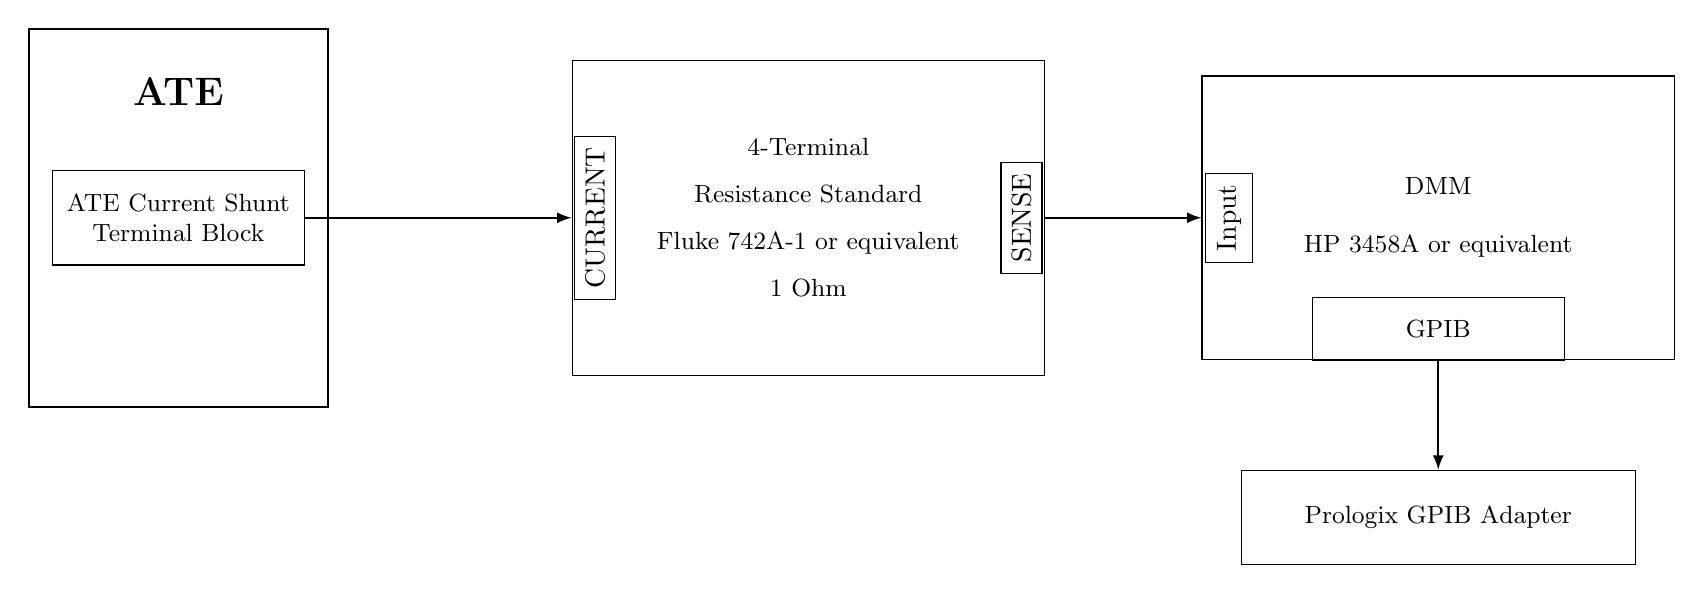
\begin{tikzpicture}[
			>=latex,
			chassis/.style={
				draw,
				rectangle,
				line width=0.8pt,
				align=center
			},
			module/.style={
				draw,
				rectangle,
				minimum width=2.5cm,
				minimum height=0.75cm,
				align=center,
				font=\small
			},
			block/.style={
				draw,
				rectangle,
				minimum width=3.0cm,
				minimum height=1.0cm,
				align=center,
				font=\small
			},
			shuntblock/.style={
				draw,
				rectangle,
				minimum width=4cm,
				minimum height=1.4cm,
				align=center,
				font=\small
			}
			]
			
			% ==================================================
			% ATE CHASSIS
			% ==================================================
			\node[
			chassis,
			minimum width=3.8cm,   % restored original width
			minimum height=4.8cm
			] (ate) at (6.0,-7.4) {};
			
			\node[font=\Large\bfseries] at (6.0,-5.8) {ATE};
			
			% ATE Current Shunt block inside chassis
			\node[
			shuntblock,
			minimum width=3.2cm,   % restored original inner width
			minimum height=1.2cm
			] (ate_shunt) at (6.0,-7.4)   % moved up for horizontal arrow
			{
				ATE Current Shunt\\
				Terminal Block
			};
			
			% ==================================================
			% RESISTANCE STANDARD
			% ==================================================
			\node[
			block,
			minimum width=6cm,
			minimum height=4cm,
			inner sep=12pt
			] (resistor) at (14.0,-7.4)
			{
				4-Terminal\\[6pt]
				Resistance Standard\\[6pt]
				\quad Fluke 742A-1 or equivalent\quad\mbox{}\\[6pt]
				1 Ohm
			};
			
			% ==================================================
			% DMM
			% ==================================================
			\node[
			block,
			minimum width=6cm,
			minimum height=3.6cm
			] (dmm) at (22.0,-7.4)
			{
				DMM\\[10pt]
				HP 3458A or equivalent
			};
			
			% GPIB block INSIDE DMM
			\node[
			draw,
			rectangle,
			minimum width=3.2cm,
			minimum height=0.8cm,
			font=\small
			] (gpib) at ($(dmm.south)+(0,0.4)$)
			{GPIB};
			
			% ==================================================
			% PROLOGIX
			% ==================================================
			\node[
			draw,
			rectangle,
			minimum width=5cm,
			minimum height=1.2cm,
			font=\small
			] (prologix) at ($(dmm.south)+(0,-2.0)$)
			{Prologix GPIB Adapter};
			
			\draw[->, thick] (gpib.south) -- (prologix.north);
			
			% ==================================================
			% SIDE LABELS
			% ==================================================
			\node[
			draw,
			rotate=90,
			fill=white,
			inner sep=4pt
			]
			at ($(resistor.west)+(0.3,0)$)
			{CURRENT};
			
			\node[
			draw,
			rotate=90,
			fill=white,
			inner sep=4pt
			]
			at ($(resistor.east)+(-0.3,0)$)
			{SENSE};
			
			\node[
			draw,
			rotate=90,
			fill=white,
			inner sep=4pt
			]
			at ($(dmm.west)+(0.35,0)$)
			{Input};
			
			% ==================================================
			% MEASUREMENT CHAIN CONNECTIONS
			% ==================================================
			\draw[->, thick] (ate_shunt.east) -- (resistor.west);
			\draw[->, thick] (resistor.east) -- (dmm.west);
			
		\end{tikzpicture}%
	}
	\caption{ATE $\rightarrow$ DMM Current Loop}
\end{figure}

\subsection{Tuning Boards}
	The ATE contains four Tuning Board sockets, one per channel. Tuning boards must be installed for each channel under test.\\\\ The tuning boards must be matched to the PSC configuration. Each channel's tuning board must be installed as a counterpart to the burdens and comps installed in the PSC, as it simulates the response of the magnet load.
	\begin{figure}[H]
		\centering
		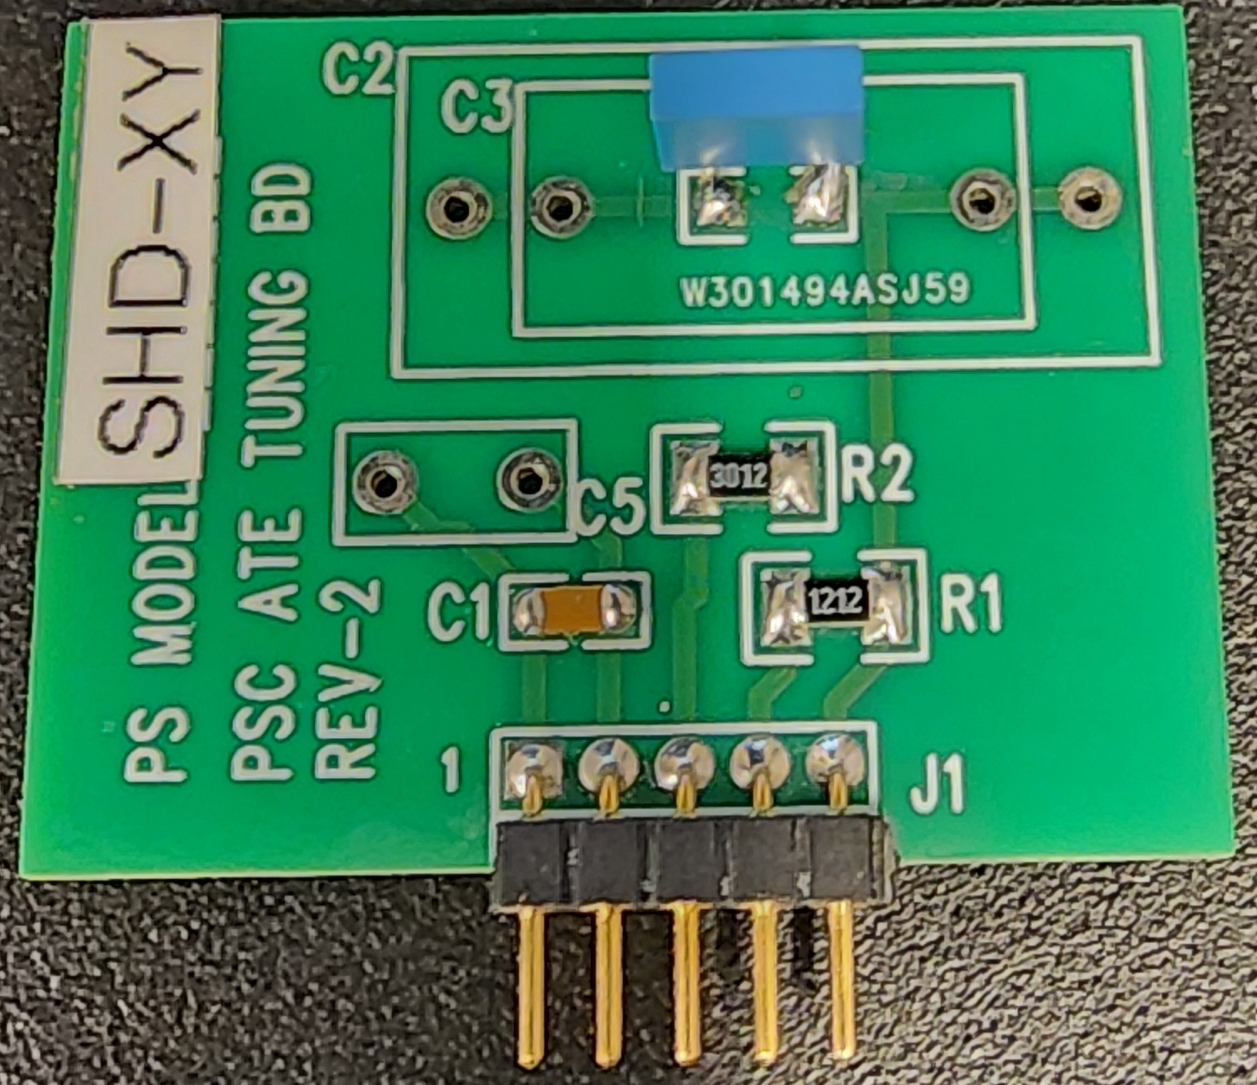
\includegraphics[width=3in]{Pictures/Tuning_Board}
		\caption{ATE Tuning Board for the ALSu SHD-XY Magnet}
	\end{figure}
    % !TeX root = ../main.tex
\chapter{zPSC Chassis Overview}
\label{chap:chassis_overview}

\section{Introduction}

\section{Front Panels (2- and 4-Channel PSCs)}
Both 2- and 4-Channel units share identical front panels:
\begin{figure}[H]
	\centering
	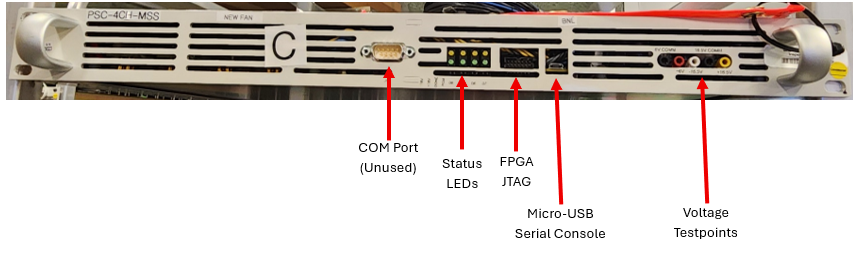
\includegraphics[width=\textwidth]{Pictures/PSC_FP_Annotated}
\end{figure}

\section{Rear Panel - 2 Channel}
\begin{figure}[H]
	\centering
	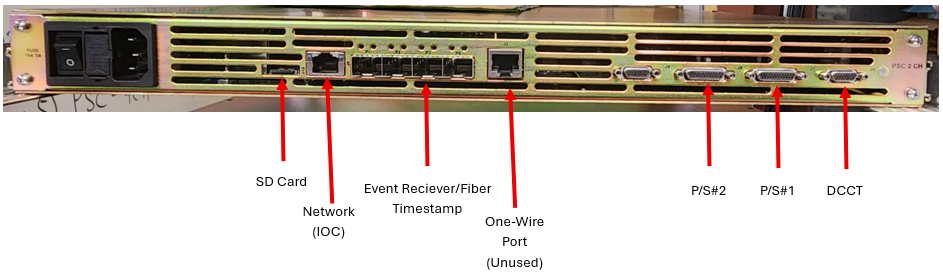
\includegraphics[width=\textwidth]{Pictures/2Ch_PSC_Annotated}
\end{figure}

\section{Internal Component Layout - 2 Channel}
\begin{figure}[H]
	\centering
	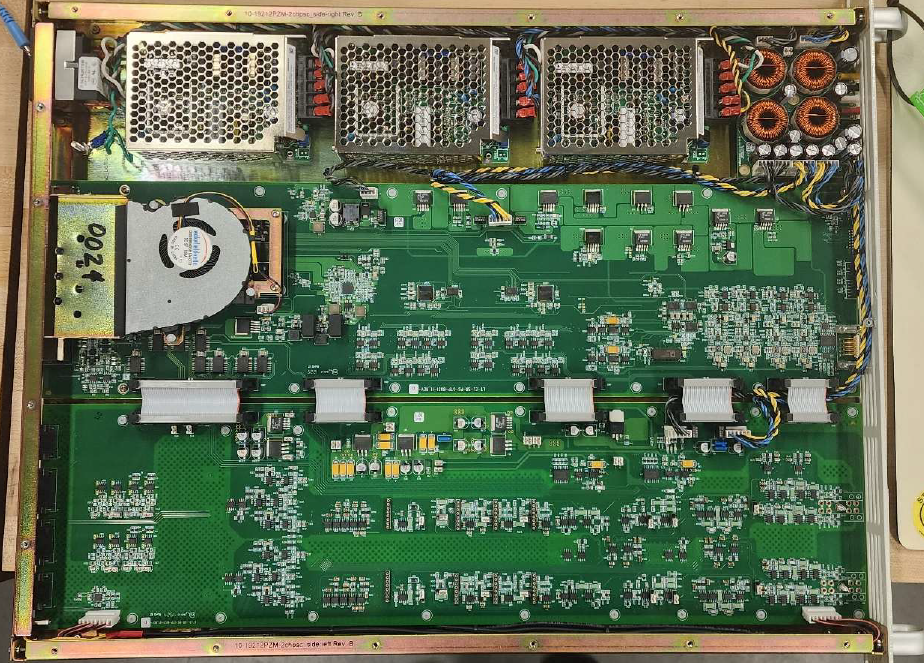
\includegraphics[width=\textwidth]{Pictures/2Ch_PSC_Chassis}
\end{figure}

\subsection{Analog Board Components}
\begin{figure}[H]
	\centering
	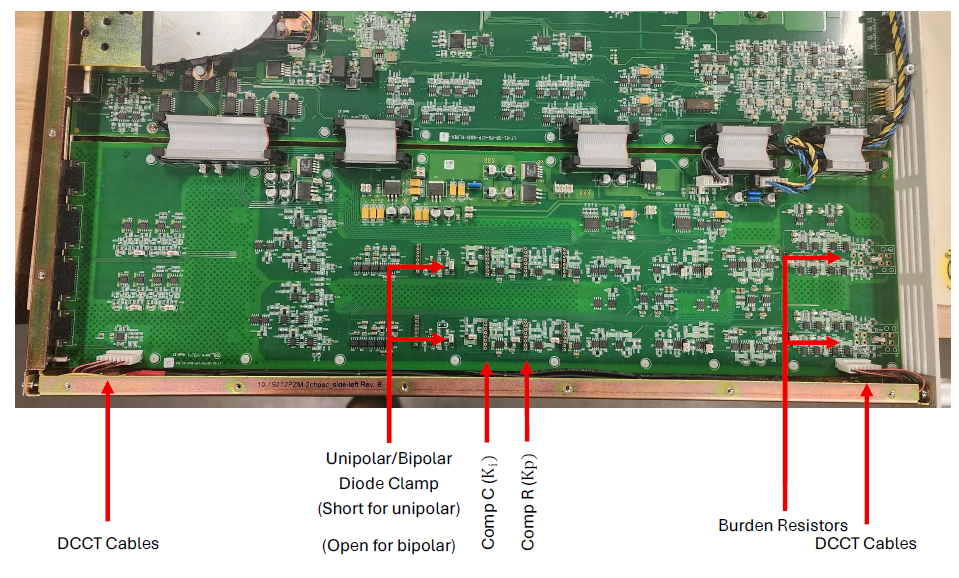
\includegraphics[width=\textwidth]{Pictures/2Ch_PSC_Analog_Brd_Annotated}
\end{figure}

\newpage
\section{Rear Panel - 4 Channel}
\begin{figure}[H]
	\centering
	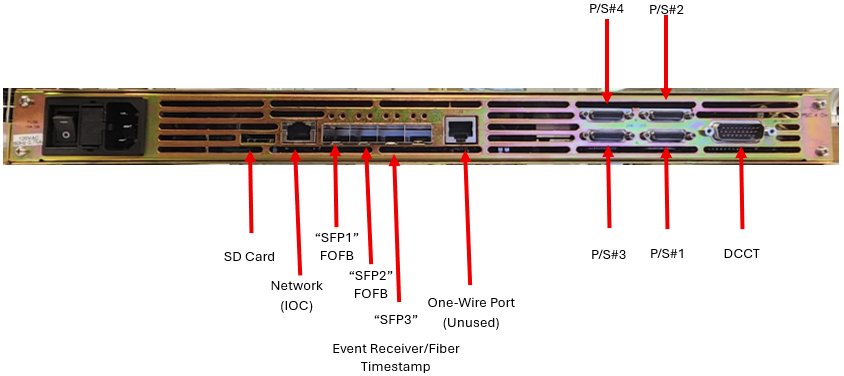
\includegraphics[width=\textwidth]{Pictures/4Ch_PSC_Rear_Annotated}
\end{figure}

\section{Internal Component Layout - 4 Channel}
\begin{figure}[H]
	\centering
	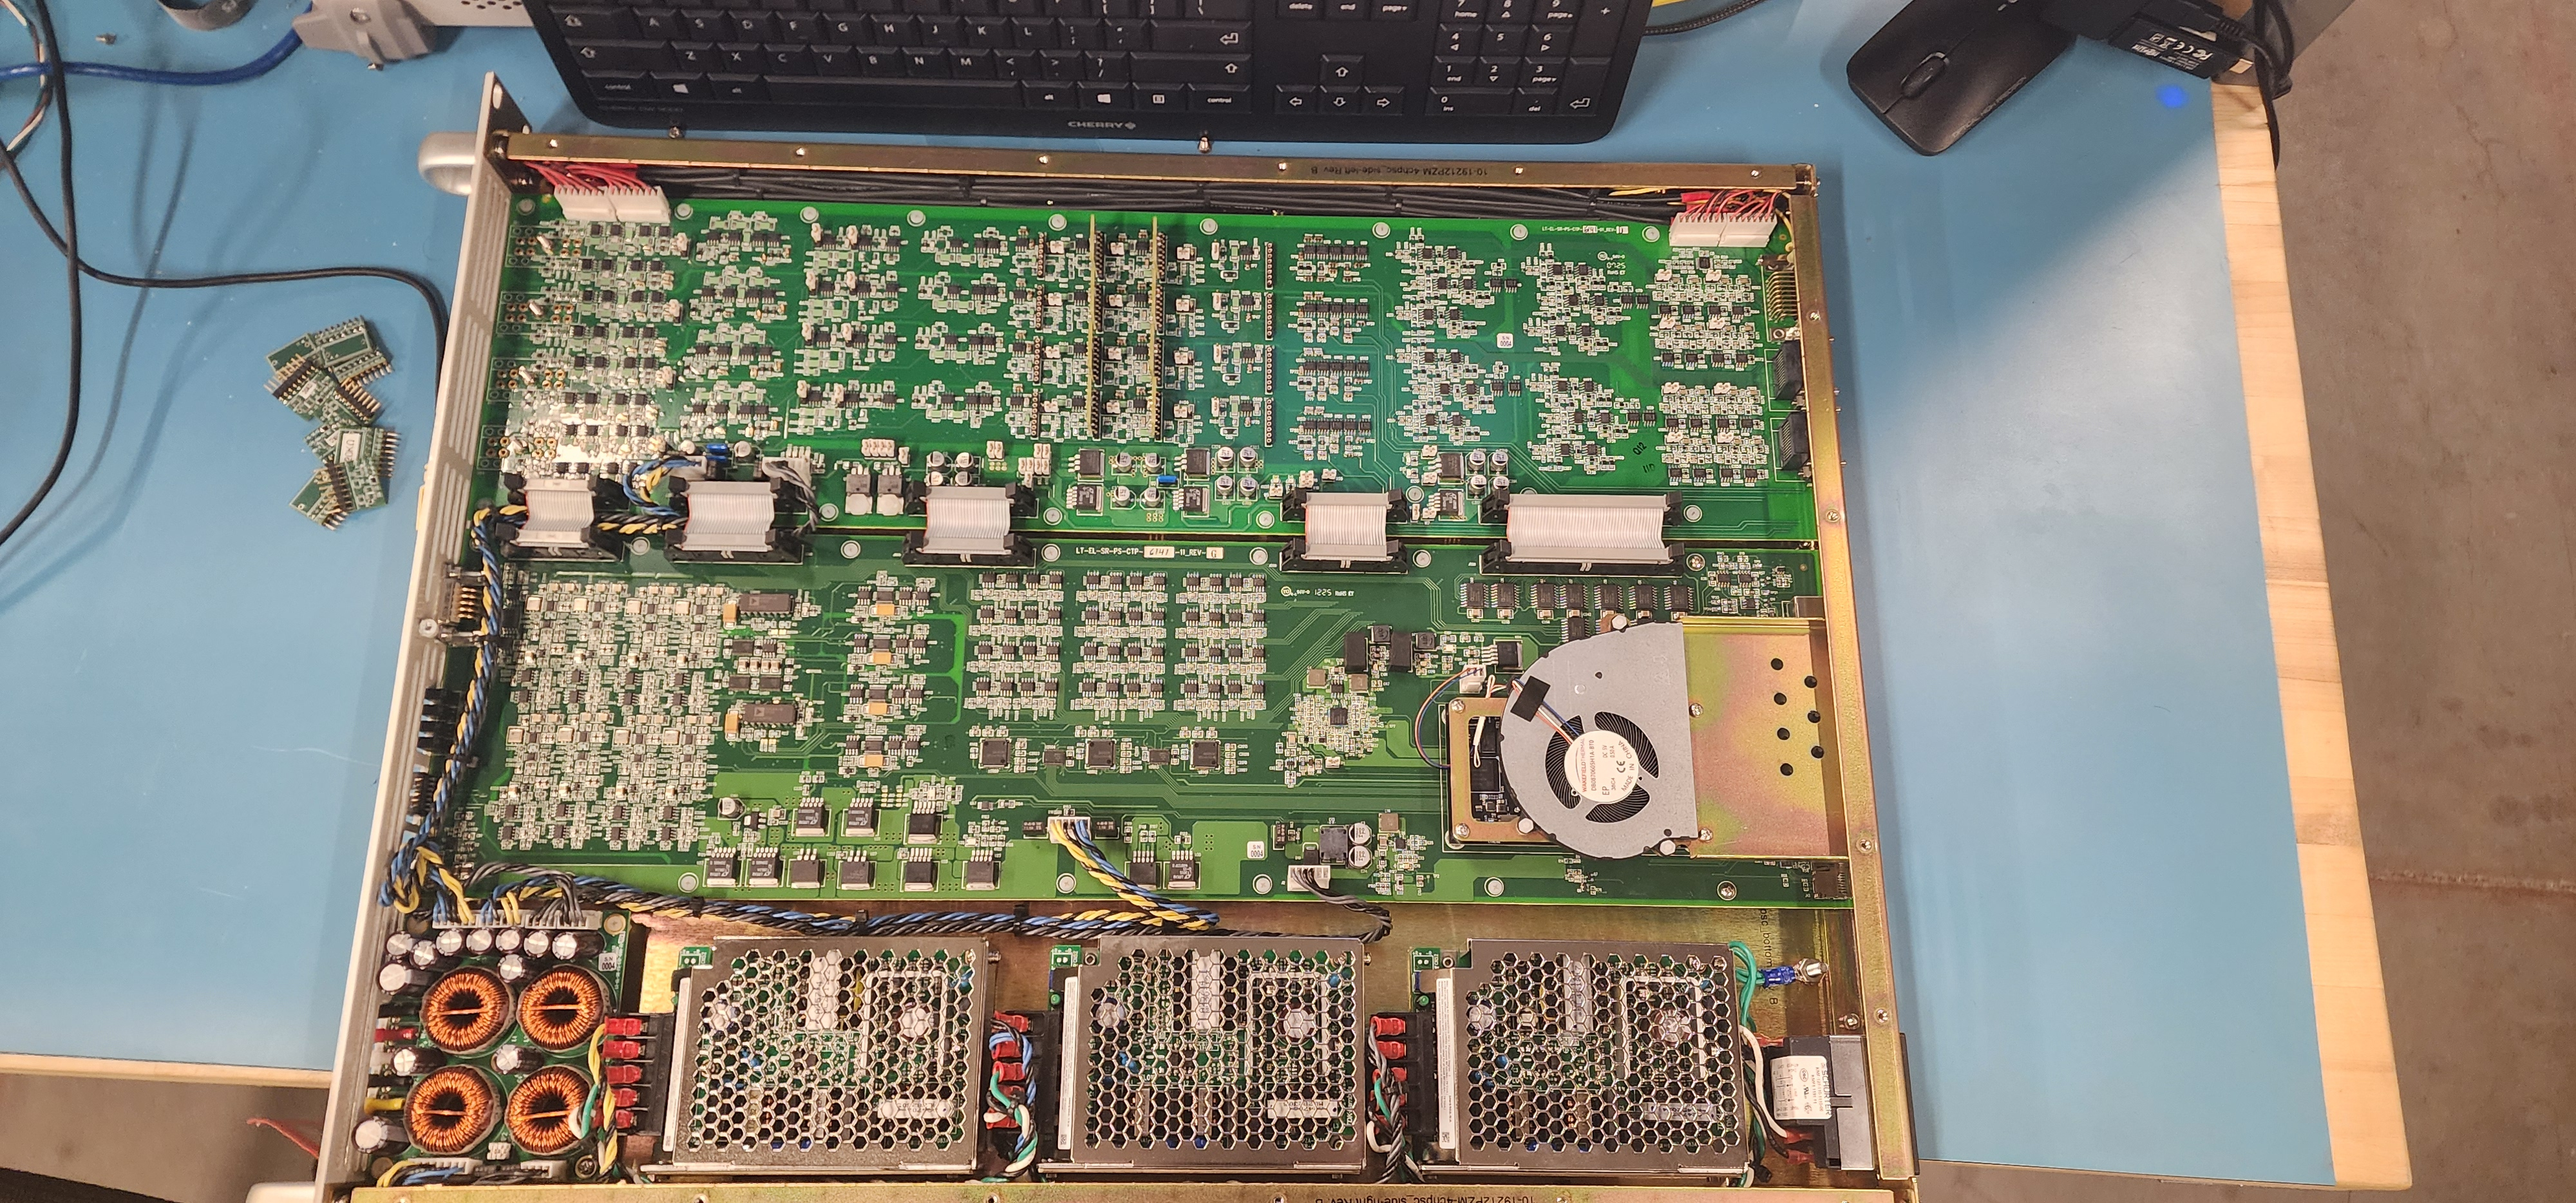
\includegraphics[width=\textwidth]{Pictures/4-Ch_PSC_Top_View}
\end{figure}

\subsection{Analog Board Components}
\begin{figure}[H]
	\centering
	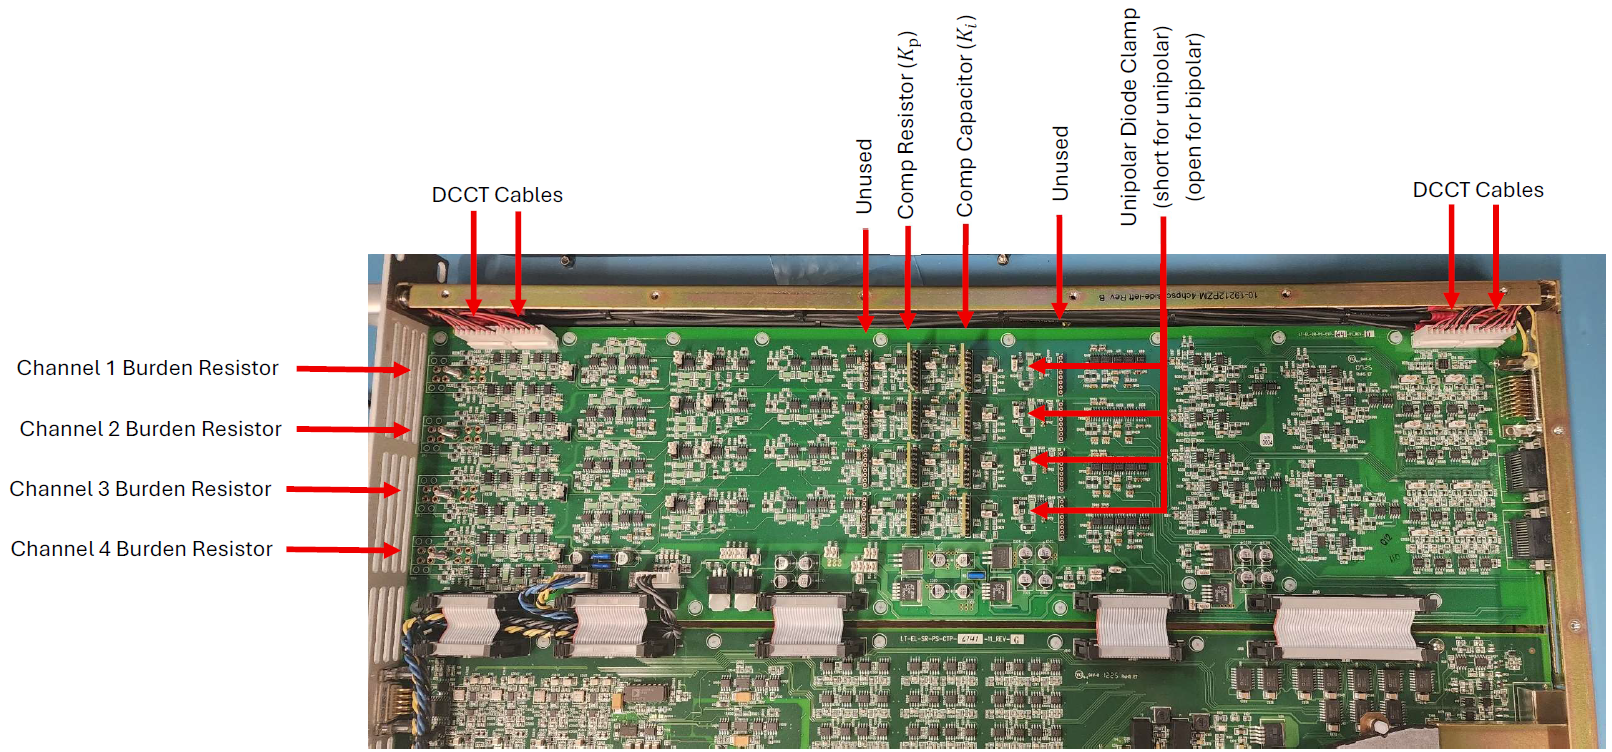
\includegraphics[width=\textwidth]{Pictures/4Ch-PSC_Analog_Brd_Annotated}
\end{figure}


    % !TeX root = ../main.tex
\chapter{EPICS Base and IOCs}
\label{chap:epics_iocs}

\section{Introduction}
There are two IOCs associated with the calibration and test of the zPSC: The ATE IOC, and the zPSC IOC.

\section{EPICS Installation Overview}
	EPICS installations performed by M. Capotosto loosely follow the below directory structure:

	\begin{itemize}
		\item \texttt{EPICS\_BASE=/epics/base} or \texttt{/epics/base\_[version]} or similar
		\item \texttt{SUPPORT=/epics/support} -- or sometimes MODULES instead of SUPPORT is used.
			\par\bigskip
			\quad Modules required for the ATE and PSC are installed here:
			\begin{itemize}[topsep=0pt]
				\item seq: SNL-Sequencer
				\item pscdrv: Portable Streaming Controller Driver
				\item asyn: EPICS module for driver and device support
			\end{itemize}
		\item \texttt{epics/iocs} - each IOC is cloned into this repository
		\item \texttt{epics/systemd-softioc} - This is an NSLS-II utility for managing IOCs as a system service
	\end{itemize}

\section{Installing EPICS Base and Required Modules}
	\begin{enumerate}
		\item Install Dependencies for Build
			\hspace*{2em} Install git, build-essential, and perl:\\ \texttt{sudo apt -y install git build-essential perl libtirpc-dev re2c libevent-dev autoconf automake libtool pkg-config}
		\item Create the EPICS user group, and the empty EPICS directory: \\
			\hspace*{2em} \texttt{sudo groupadd epics}\\
			\hspace*{2em} \texttt{sudo usermod -aG epics \$USER}\\
			\hspace*{2em} \texttt{newgrp epics}\\
			\hspace*{2em} \texttt{sudo mkdir -p /epics}\\
			\hspace*{2em} \texttt{sudo chown \$USER:epics /epics}\\
			\hspace*{2em} \texttt{sudo chmod 2775 /epics}\\
		\item EPICS Base is cloned into \texttt{/epics/base} via:\\
			\hspace*{2em} \texttt{git clone --recursive -b 7.0} \\ \hspace*{4em}\texttt{https://github.com/epics-base/epics-base.git /epics/base}\\
			\hspace*{2em} \texttt{cd /epics/base}\\

            \textbf{Note:} The \texttt{7.0} branch tracks ongoing EPICS Base development and may contain commits newer than the most recent stable release. During testing, the development branch produced a Channel Access regression that caused \texttt{caput} operations to disconnect from the IOC. EPICS Base was therefore pinned to the stable \texttt{R7.0.10} release tag before building:

            \hspace*{2em} \texttt{git checkout R7.0.10}

            \hspace*{2em} \texttt{git submodule update --init --recursive}
		\item Build EPICS:\\
			\hspace*{2em} \texttt{make clean}\\
			\hspace*{2em} \texttt{make}\\

        \item Add the EPICS Base binaries to the user's PATH:\

            \hspace*{2em} \texttt{echo 'export EPICS\_BASE=/epics/base' >> \textasciitilde/.bashrc}\

            \hspace*{2em} \texttt{echo 'export EPICS\_HOST\_ARCH=linux-x86\_64' >> \textasciitilde/.bashrc}\

            \hspace*{2em} \texttt{echo 'export PATH=\$EPICS\_BASE/bin/\$EPICS\_HOST\_ARCH:\$PATH' >>    \textasciitilde/.bashrc}\

            \hspace*{2em} \texttt{source \textasciitilde/.bashrc}\

		\item Create the remaining directory structure:\\
			\hspace*{2em} \texttt{mkdir -p /epics/iocs /epics/modules}\\

		\item Clone asyn:
			\begin{enumerate}
				\item \texttt{cd /epics/modules}
				\item \texttt{git clone https://github.com/epics-modules/asyn.git asyn}
				\item \texttt{cd /epics/modules/asyn}
				\item Set up required files in \texttt{configure/RELEASE, configure/RELEASE.LOCAL}
				\item Build with \texttt{make clean}, and \texttt{make}
			\end{enumerate}

		\item Clone Sequencer:
		\begin{enumerate}
			\item \texttt{cd /epics/modules}
			\item \texttt{git clone https://github.com/epics-modules/sequencer.git seq}
			\item \texttt{cd /epics/modules/seq}
			\item Set up required files in \texttt{configure/RELEASE, configure/RELEASE.LOCAL}
			\item Build with \texttt{make clean}, and \texttt{make}
		\end{enumerate}

		\item Clone PSC Driver:
		\begin{enumerate}
			\item \texttt{cd /epics/modules}
			\item \texttt{git clone https://github.com/mdavidsaver/pscdrv.git pscdrv}
			\item \texttt{cd /epics/modules/pscdrv}
			\item Set up required files in \texttt{configure/RELEASE, configure/RELEASE.LOCAL}
			\item Build with \texttt{make clean}, and \texttt{make}
		\end{enumerate}

		\item Clone Manage IOCs Utility:
		\begin{enumerate}
			\item \texttt{cd /epics}
			\item \texttt{git clone https://github.com/NSLS2/systemd-softioc.git}
			\item Navigate to the repo directory \texttt{cd systemd-softioc}
			\item Make the install script executable and run:\\
			\hspace*{2em}\texttt{sudo chmod +x install.sh}\\
			\hspace*{2em}\texttt{sudo ./install.sh}\\
			\hspace*{2em}\texttt{sudo usermod -aG epics softioc}\\
			\hspace*{2em}\texttt{newgrp}\\
			\hspace*{2em}\texttt{sudo chown softioc:epics /epics/iocs}\\
			\hspace*{2em}\texttt{sudo chmod 2775 /epics/iocs}\\
		\end{enumerate}
	\end{enumerate}

\section{Installing the ATE IOC}
	\begin{enumerate}
		\item Change to IOC directory \texttt{cd /epics/iocs}
		\item Clone the repo:\\
		\hspace*{1em} \texttt{git clone https://github.com/capotosto/ALSu-PSC\_ATE-ioc.git PSCtest}
		\item \texttt{cd PSCtest}
		\item \texttt{git switch Released,-UPC/BPC-Split-IOC-Ver-2}
		\item Create the \texttt{RELEASE.local} file, \texttt{touch configure/RELEASE.local}
		\item \texttt{echo -e "EPICS\_BASE=/epics/base\textbackslash nASYN=/epics/modules/asyn" >}\\
			\hspace*{2em} \texttt{ /epics/iocs/PSCtest/configure/RELEASE.local}
		\item Build the IOC: \texttt{make clean}, \texttt{make}
		\item Update the st.cmd file: \texttt{cd iocBoot/iocPSCtest}
			\begin{enumerate}
			\item Edit the st.cmd file: \texttt{nano st.cmd}
			\item Update the EPICS\_BASE variable if needed.
			\item Update the IPPORT to match the ATE. Repository has 10.69.26.4:5000 as default. Changing this later from the Phoebus/CSS panels may not work!
		\end{enumerate}

		\item Find the next available port: \texttt{manage-iocs nextport}
		\item Configure this in the config file: \texttt{nano config}
		\item Set the \texttt{NAME=PSCtest}, \texttt{PORT=} your next port, \texttt{USER=softioc}, and \texttt{HOST=\$HOSTNAME}
		\item Update the directory path in the root-level st.cmd to point to the right binaries
		\item Enroll in manage-iocs as a service: \texttt{sudo manage-iocs install PSCtest}
		\item Enable auto-start on boot: \texttt{sudo manage-iocs enable PSCtest}
		\item Check the status, it should be running! \texttt{manage-iocs status}
		\item And if you want other information on the ioc: \texttt{manage-iocs report}
	\end{enumerate}

\section{Installing the PSC IOC}
\begin{enumerate}
	\item Change to IOC directory \texttt{cd /epics/iocs}
	\item Clone the repo:\\
	\hspace*{1em} \texttt{git clone https://github.com/jamead/zpsc-ioc.git zpsc\_ioc}
	\item \texttt{cd zpsc\_ioc}
	\item Create the \texttt{RELEASE.local} file, \texttt{touch configure/RELEASE.local}
	\item \texttt{echo -e "EPICS\_BASE = /epics/base\textbackslash n}\\
		\hspace*{2em}\texttt{PSCDRV = /epics/modules/pscdrv\textbackslash n}\\
		\hspace*{2em}\texttt{SEQ = /epics/modules/seq" >}\\
		\hspace*{2em} \texttt{/epics/iocs/zpsc\_ioc/configure/RELEASE.local}
	\item Build the IOC: \texttt{make clean}, \texttt{make}
	\item Update the st.cmd file as needed: \texttt{cd iocBoot/ioczpsc}
	\item Create the st.cmd file used by systemd-softioc: \begin{verbatim}echo -e '#!/bin/bash\n\n
		cd "/epics/iocs/zpsc_ioc/iocBoot/ioczpsc"\n./st.cmd' > st.cmd\end{verbatim}
	\item Make the new st.cmd executable: \texttt{chmod +x st.cmd}
	\item Find the next available port: \texttt{manage-iocs nextport}
	\item Configure this in the config file: \texttt{nano config}
	\item Set the \texttt{NAME=zpsc\_ioc}, \texttt{PORT=} your next port, \texttt{USER=softioc}, and \texttt{HOST=\$HOSTNAME}
	\item Update the directory path in the root-level st.cmd to the \texttt{iocBoot/ioczpsc/st.cmd}
	\item Enroll in manage-iocs as a service: \texttt{sudo manage-iocs install zpsc\_ioc}
	\item Enable auto-start on boot: \texttt{sudo manage-iocs enable zpsc\_ioc}
	\item Check the status, it should be running! \texttt{manage-iocs status}
	\item And if you want other information on the ioc: \texttt{manage-iocs report}
\end{enumerate}





















    % !TeX root = ../main.tex
\FloatBarrier
\chapter{CS-Studio - Phoebus}
\label{chap:cs-studio}

\section{Introduction}
CS-Studio Phoebus is installed using precompiled binaries. This application requires a Java runtime environment be installed.\\

\noindent The 'BOB' files - the user interface panels, are located in the IOC's directories, \path{/epics/iocs/PSCtest/gui} and \texttt{/epics/iocs/zpsc\_ioc/gui}\\

\noindent Behavior of some features of Phoebus must be modified by the shell script used to launch Phoebus, an example is included with the below installation instructions to modify the behavior of the 'Home' button, used to bring up the custom 'PSC Launcher' panel using the Home button, instead of having to manually navigate to the file when needed.\\

\section{Installing Phoebus}
\begin{enumerate}
	\item If not installed, install Java, e.g.:\\
		\hspace*{2em}\texttt{sudo apt update \&\& sudo apt install openjdk-17-jdk}
	\item Create the directory: \texttt{sudo mkdir /opt/phoebus}\\
		\hspace*{2em}\texttt{chown \$USER:epics /opt/phoebus}\\
		\hspace*{2em}\texttt{chmod 2775 /opt/phoebus}
	\item Download Phoebus and extract to the \texttt{/opt/phoebus} directory\\
	\href{https://github.com/ControlSystemStudio/phoebus/releases/download/v4.7.4/phoebus-4.7.4-linux.tar.gz}{https://github.com/ControlSystemStudio/phoebus/releases/download/v4.7.4/phoebus-4.7.4-linux.tar.gz}
	\item{Make the shell script executable: \texttt{chmod +x phoebus.sh}}
	\item Copy in necessary configuration changes from the template:\\
		\hspace*{2em}\texttt{git clone }\\
		\hspace*{2em}\texttt{https://github.com/capotostobnl/Phoebus-ALSU.git /opt/phoebus/config}
	\item Update paths as necessary in the \texttt{settings.in}/\texttt{settings\_template.ini}
	\item Alias Phoebus to run via command \texttt{run-phoebus}:\\
		\hspace*{2em}\texttt{echo 'alias run-phoebus="/opt/phoebus/phoebus.sh"' >> ~/.bashrc}\\
		\hspace*{2em}\texttt{source \textasciitilde/.bashrc}
	\item{Now test! Try run-phoebus from a terminal, and then click the 'Home' button!}
	
	\end{enumerate}

    % !TeX root = ../main.tex

\chapter{Networking}
\label{chap:Networking}
\section{Overview}
The default configuration for these devices is to use static IP addresses on the 10.69.26.0/23 subnet.\\\\
The network topology is generally as follows: 
\begin{figure}[htbp]
	\centering
	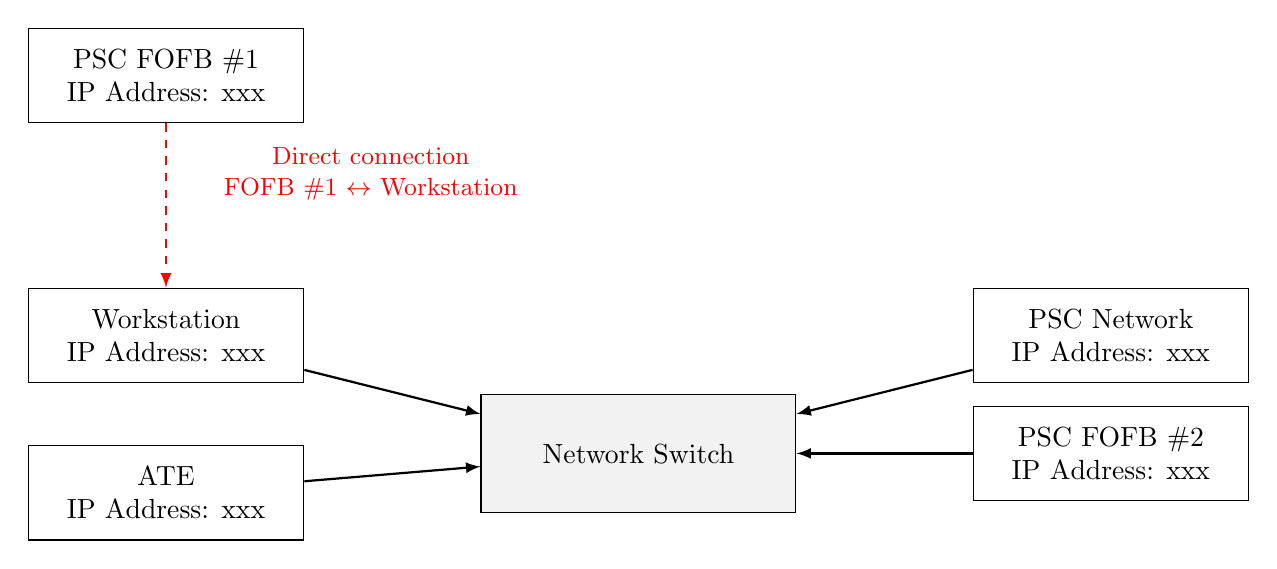
\begin{tikzpicture}[
		node/.style={draw, rectangle, minimum width=3.5cm, minimum height=1.2cm, align=center},
		switch/.style={draw, rectangle, minimum width=4cm, minimum height=1.5cm, fill=gray!10, align=center},
		line/.style={-latex, thick}
		]
		
		% ======================
		% Network Switch
		% ======================
		\node[switch] (sw) at (0,0) {Network Switch};
		
		% ======================
		% LEFT SIDE
		% ======================
		\node[node] (workstation) at (-6,1.5) {Workstation\\IP Address: xxx};
		
		\node[node] (ate) at (-6,-0.5) {ATE\\IP Address: xxx};
		
		\node[node] (fofb1) at (-6,4.8) {PSC FOFB \#1\\IP Address: xxx};
		
		% ======================
		% RIGHT SIDE
		% ======================
		\node[node] (pscnet) at (6,1.5) {PSC Network\\IP Address: xxx};
		
		\node[node] (fofb2) at (6,0) {PSC FOFB \#2\\IP Address: xxx};
		
		% ======================
		% CONNECTIONS
		% ======================
		\draw[line] (workstation) -- (sw);
		\draw[line] (ate) -- (sw);
		\draw[line] (pscnet) -- (sw);
		\draw[line] (fofb2) -- (sw);
		
		% ======================
		% DIRECT CONNECTION
		% ======================
		\draw[line, dashed, red, thick] (fofb1) -- (workstation);
		
		\node[red, font=\small, align=center]
		at ($(fofb1)!0.5!(workstation) + (2.6,0.4)$)
		{Direct connection\\FOFB \#1 $\leftrightarrow$ Workstation};
		
	\end{tikzpicture}
	\caption{Network Topology with Clean FOFB Direct Link}
\end{figure}
    % !TeX root = ../main.tex

\chapter{Installing Minicom}
\label{chap:Installing Minicom}
\section{Overview}
    % !TeX root = ../main.tex

\chapter{Python Installation and Configuration}
\label{chap:Python Installation and Configuration}
\section{Overview}
Python3 is required for the calibration and test scripts to be run for the PSCs. Below sections will describe the process for installing Python3, and handling package management and virtual environment management, if desired. 

\section{Installing and Configuring Python, and the Python Environment}
\subsection{Installing Python}
Many downstream Debian-based distributions come bundled with Python3. If yours does not, install Python3 via: \texttt{sudo apt update \&\& sudo apt install python3}

\subsection{Python Package Management}
\subsubsection*{Installing Pip}
These scripts were written using Python3. It is assumed that Python3 is already installed on your workstation.\\\\
A Pip requirements file is included in the repository for ease of package management, but pip may not come bundled with the OS; to install Pip:\\
\texttt{sudo apt install python3-pip}

\subsubsection*{Installing Packages}
Packages can be simply installed via pip now.\\\\
If within a virtual environment, use: \texttt{pip install -r requirements.txt}\\
If not using environments: \texttt{python3 -m pip install -r requirements.txt}\\
If you run into permissions issues: \texttt{python3 -m pip install --user -r requirements.txt}


\subsection*{Python Virtual Environments}
It may be desireable to use a virtual environment, e.g., venv or Conda, especially if other scripts are used on this machine that may have overlapping or conflicting packages installed. My personal preference is for venv, however Conda is used by NSLS-II at the organizational level. venv is a simpler and light weight tool, if it is needed only for running Python projects. \\\\
venv can be installed with:\\
\texttt{sudo apt install python3-venv}\\\\
The environment can then be activated with \texttt{python3 -m venv my\_venv\_name}. You can then activate the environment with \texttt{source my\_venv/bin/activate}. 


    % !TeX root = ../main.tex

\chapter{Calibration and Test Script Installation}
\label{chap:Calibration and Test Script Installation}
\section{Overview}

The repository for the calibration and test scripts can be found at: \url{https://github.com/capotostobnl/NSLS2_zPSC_Calibration_and_Test}

Details regarding the use of the script will come in the following chapters on Calibration and on Functional Tests, though all scripts are launched from this one repository's 'launcher.py' script. 

\section{Cloning the Script Repository}
	\begin{enumerate}
		\item Choose a location for the repo, and go there: \texttt{cd ~/}
		\item Clone the repository: \texttt{git clone \url{https://github.com/capotostobnl/NSLS2_zPSC_Calibration_and_Test}}
	\end{enumerate}
	
\section{Creating the Virtual Environment}
If you choose to use a virtual environment, create it and then install the dependencies. If you choose to not use venv, you can skip to installing dependencies in the next section. 
	\begin{enumerate}
		\item Navigate to the repository and then: \texttt{python3 -m venv .venv}
		\item Activate the environment: \texttt{source .venv/bin/activate}
	\end{enumerate}

\section{Installing Dependencies}
Required Python modules can be installed via the requirements.txt from the repository via: \texttt{python3 -m pip install -r requirements.txt}
    % !TeX root = ../main.tex

\chapter{Configuring the Test and Calibration Scripts}
\label{chap:Configuring the Test and Calibration Scripts}
\section{Overview}
There are many places where changes may need to be made when bringing a new workstation up for the first time.\\\\
After initial configuration, no further changes should be required, with the exception of the \texttt{psc\_models.py} class, which will be modified any time a new PSC is added, or a particular PSC's configuration requirements are changed.
\section{The \texttt{common} Files Directory}
This directory contains a number of modules which may need reconfiguration as outlined below.\\\\
Files in this directory may be used by both the Calibration side and the Test side of the script package. 

\subsection{EPICS Drivers}
There are two modules, \texttt{ate\_epics.py} and \texttt{psc\_epics.py} which provide a library of function calls to read and write various EPICS PVs. As firmware and IOC changes are made, some changes may be required in these drivers to add new features, or fix features that are removed or break.\\\\
These two modules are little more than a pyepics wrapper. 

\subsection{The \texttt{initialize\_dut.py} Utility}
This is a small utility that collects information from the PSC EEPROM, generate the filenames, timestamps, and directory structures to be used during calibration and test.
 
\subsection{The \texttt{psc\_models.py} Class}


\section{Calibration}
\subsection{The \texttt{initialize\_qspi.py} Module}

\subsection{The \texttt{psc\_calibration.py} Module}



\section{Functional Test}
    % !TeX root = ../main.tex

\chapter{Initial Booting of the PSC and Configuration of the EEPROM}
\label{chap:Initial Booting of the PSC and Configuration of the EEPROM}
\section{Overview}
This section will discuss the steps required for the first time booting a new PSC, and initializing the EEPROM.\\\\
\textbf{The EEPROM must be configured before many functions will work.}\\\\
It is important to note that once the EEPROM is configured, many parameters of the PSC will still provide inconsistent or invalid data until the QSPI values are initialized properly via the scripts outlined in \autoref{chap:Running the Calibration and Test Script}.

\subsection{Creating the SD Card}
First, a new SD card must be generated and installed in the PSC. We have been using Microcenter 32GB microSD cards, though other brands and sizes may (or may not) work.\\

\begin{enumerate}
	\item Download the BOOT.bin binaries from the git repository\\
	For convenience, the latest stable version of firmware is located in the test script repostiory outlined in \autoref{chap:Running the Calibration and Test Script}.\\\\
	Copy to your SD card this BOOT.bin
	
	\item Create and Save the NET.CNF file to the SD card\\
	A NET.CNF file is included in the repository as well, and can be used with no modifications so long as only one PSC is connected to the network at a time. Connecting more requires changing the static IP address set in this file for each PSC. 
	
	\item Eject the SD card, and install in the zPSC, it should now be ready to boot. 
	
	\item Turn on the PSC, it should boot, indicated by front panel LED D8 rapidly flashing. It may take 60 to 90 seconds for the PSC to connect to the network and ping, be patient.\\The PSC will take an extended amount of time to boot the RTOS if no ethernet cable is connected at all.  
\end{enumerate}

\subsection{Configuring the EEPROM}
Once the PSC has booted, we can proceed to writing the EEPROM configuration.\\
\begin{enumerate}
	\item Connect the micro-USB cable to the front panel port of the PSC, and identify which serial port it appears as on your terminal.\\
	You may need to do a directory list before and after plugging in, to see which serial device appears:\\
	\texttt{ls /dev}\\
	In this example, the PSC will appear as /dev/ttyUSB2.\\
	\begin{figure}[H]
		\centering
		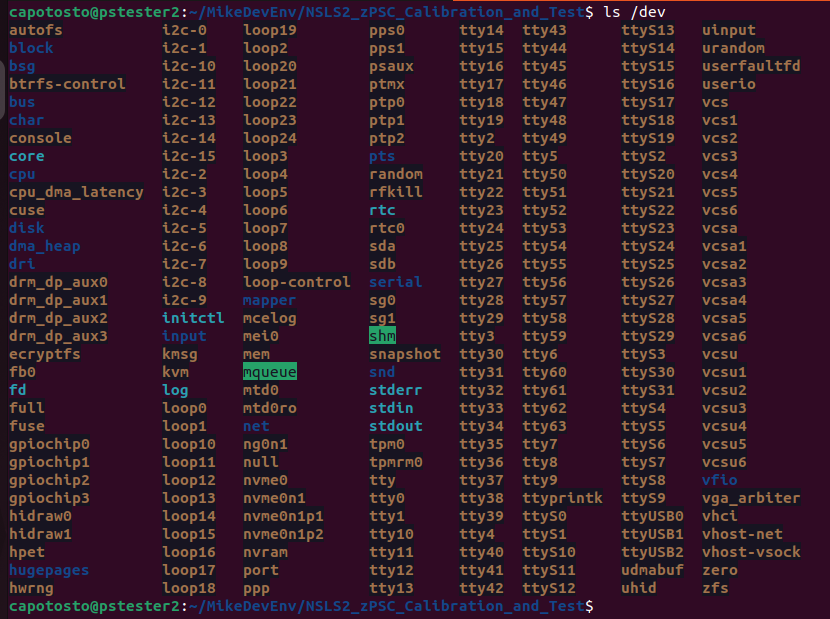
\includegraphics[width=\textwidth]{Python_Screenshots/ls_dev}
	\end{figure}
	\newpage
	\item Open Minicom using the port you determined: \texttt{minicom -D /dev/ttyUSB2}
		\begin{figure}[H]
			\centering
			\includegraphics[width=4in]{Python_Screenshots/EEPROM_Terminal}
		\end{figure}
	\item  Set Items B through E for a standard PSC, and F, G as needed.
		\begin{figure}[H]
			\centering
			\includegraphics[width=4in]{Python_Screenshots/minicom b}
			\caption{Setting B}
		\end{figure}
		\begin{figure}[H]
			\centering
			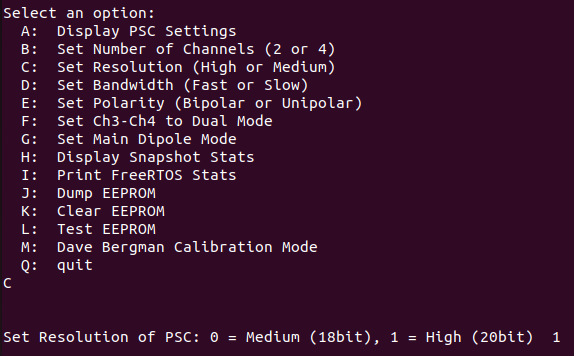
\includegraphics[width=4in]{Python_Screenshots/minicom c}
			\caption{Setting C}
		\end{figure}
		\begin{figure}[H]
			\centering
			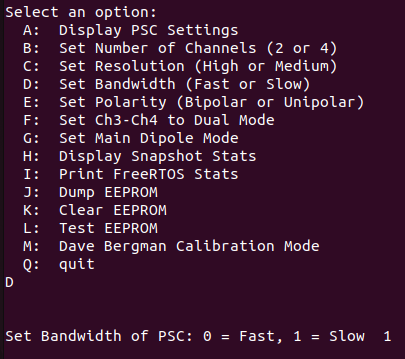
\includegraphics[width=4in]{Python_Screenshots/minicom d}
			\caption{Setting D}
		\end{figure}
		\begin{figure}[H]
			\centering
			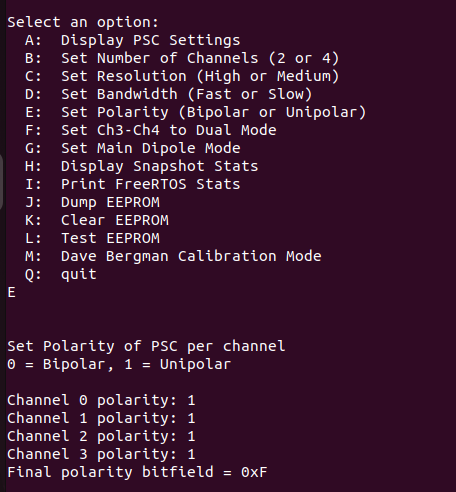
\includegraphics[width=4in]{Python_Screenshots/minicom e}
			\caption{Setting E}
		\end{figure}
	\newpage
	\item Verify the settings with Option A:
		\begin{figure}[H]
			\centering
			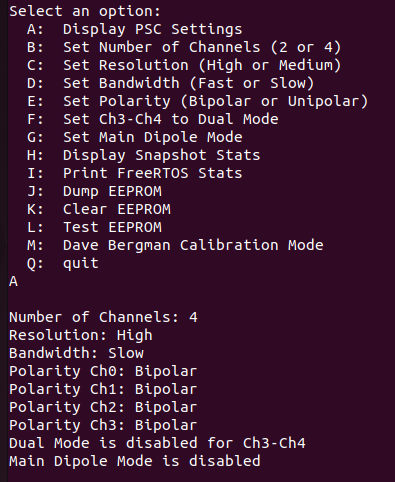
\includegraphics[width=4in]{Python_Screenshots/minicom a}
			\caption{Setting A}
		\end{figure}
	\item If satisfied, it is now safe to unplug the USB cable, no further action is necessary. To exit Minicom, press \texttt{ctrl+a}, release, press \texttt{x}, release, and finally press \texttt{<return>} for 'Yes' to exit.
\end{enumerate}
    % !TeX root = ../main.tex

\chapter{Running the Calibration and Test Script}
\label{chap:Running the Calibration and Test Script}
\section{Overview}

This section will describe how to run and use the Calibration and Test Script, assuming it is configured properly. The following chapters will go into detail on adding new PSC models, and specific details regarding the calibration side and test side of the scripts. 

\begin{center}
	\setlength{\fboxrule}{1.5pt}
	\setlength{\fboxsep}{6pt}
	\fbox{
		\parbox{0.9\textwidth}{
			\textbf{The EEPROM must be configured in the PSC prior to using any of these scripts. Failure to configure the EEPROM, or incorrectly configuring it, will cause issues with the script at even the first menu selection stages.}
		}
	}
\end{center}

\section{Running the Script: Launcher Menu}
To run the script, simply execute the launcher.py script from the repository root directory: \texttt{python3 launcher.py}\\
A menu will appear in your terminal. 
\begin{figure}[H]
	\centering
	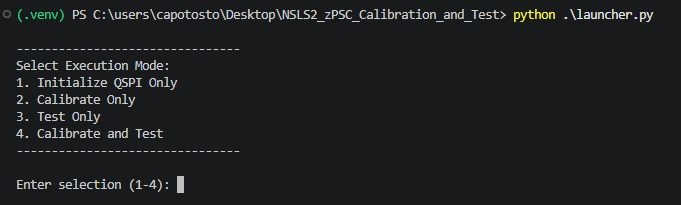
\includegraphics[width=\textwidth]{Python_Screenshots/launcher_menu}
\end{figure}

\newpage \textbf{Choose an option from the menu.}
\begin{enumerate}
	\item Initialize QSPI Only\\
	This option will set the QSPI parameters normally written at the end of calibration, so values such as OVP/OCP, scale factors, and such, will be written to the flash. All gains are written as 1.00, and all offsets written as 0.0. This will overwrite any values stored in QSPI!\\\\This is especially useful for initial testing, where you may want to verify all channels work visually, before committing the time to calibrate and test.
	
	\item Calibrate Only\\
	This option will perform a calibration only, without any tests. This will write all QSPI values at the end of the calibration for each channel.
	
	\item Test Only\\
	This option will perform only the functional tests, without a calibration. This makes no changes to the QSPI. 
	
	\item Calibrate and Test\\
	This option will run a full calibration, and immediately upon completion of the calibration, it will begin the functional test. This allows a calibration and test cycle to be started, and then left alone; so long as the calibration doesn't fail in a way that exits the script, the test can be left unattended for the duration and it will complete without any further user input once it has began (with the exception of the Fast Orbit Feedback Test, which requires a user password)
\end{enumerate}

\newpage
\subsection{Option 1: Initialize QSPI Only}
An example screenshot is provided below.\\
After selecting Menu Option 1, Initialize QSPI Only, the script will sweep the network to detect PSCs. If only one PSC pings, it'll automatically select this unit. If it times out, it'll prompt for the PV prefix of the PSC.\\

The script reads the EEPROM configuration, and trims the option list to those PSCs that match the EEPROM.\\

In this example, a 4Ch High-Stability Fast EIC PSC was being configured, so we chose Option 4. Each channel's QSPI was then written, and the script exited gracefully. 

\begin{figure}[H]
	\centering
	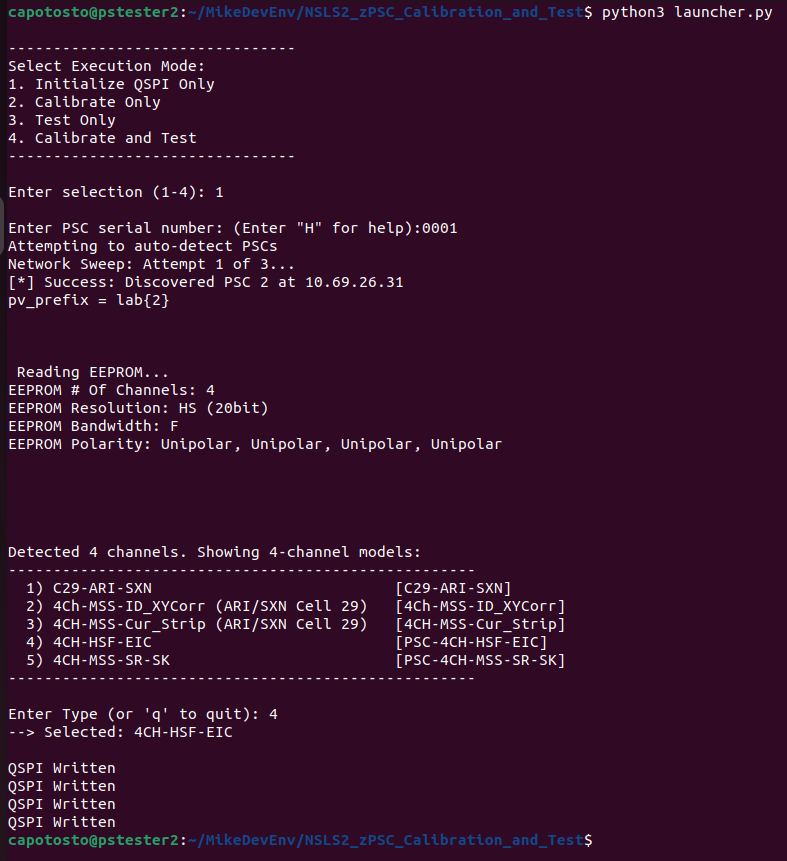
\includegraphics[width=5.75in]{Python_Screenshots/Initialize_QSPI}
\end{figure}
\newpage

\subsection{Option 2: Calibrate Only}
An example screenshot is provided below.\\
After selecting Menu Option 2, Calibrate Only, the script will sweep the network to detect PSCs. If only one PSC pings, it'll automatically select this unit. If it times out, it'll prompt for the PV prefix of the PSC.\\\\
The script reads the EEPROM configuration, and trims the option list to those PSCs that match the EEPROM.\\\\
In this example, a 4Ch High-Stability Slow PSC was being calibrated, so we chose Option 5.\\

A few new prompts will appear:
\begin{enumerate} 
	\item How long do you want to sleep before beginning? (Minutes):\\
	This is asking how long to delay the script's start. For example, if you want the script to wait 15 minutes for the unit to warm up and thermally stabilize, you can simply type 15 and hit \texttt{return}. The script will wait 15 minutes, and then start automatically. 
	
	\item Are the correct tuning boards installed in the ATE? $<$Y/N$>$:\\
	This is a reminder to check and install the correct tuning boards in the ATE. This does not have any effect on the script's function - it does not perform any self tests or verification! It is simply a reminder. Incorrect tuning boards will cause the unit to behave unpredictably.\\
	Install the correct tuning boards before proceeding.
	
	\item Have you run the DMM Self-Calibration within the last 8 hours? $<$Y/N$>$:\\
	This is another reminder prompt. If you haven't, simply perform the auto-cal on the DC Volts range before proceeding. 
	
	\item The calibration script will now take the reigns from here. No further user input is required, the calibration will run, printing results to the terminal as it progresses. Once it completes, it will automatically generate a report text file, timestamped with the model and serial number of the PSC in the filename, located in the \texttt{/cal\_reports} directory. 
\end{enumerate}

\begin{figure}[H]
	\centering
	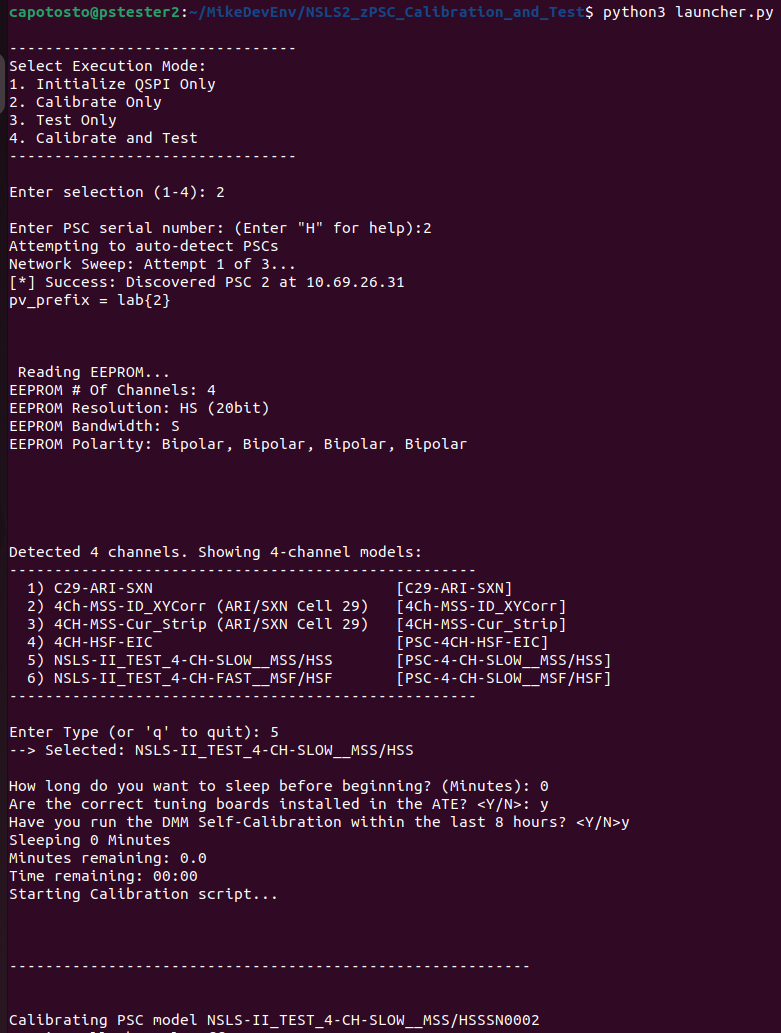
\includegraphics[width=6in]{Python_Screenshots/Calibration_Launch}
	\caption{Menu to launch a Calibrate Only calibration of a PSC}
\end{figure}

\newpage
\subsection{Option 3: Test Only}
An example screenshot is provided below.\\
After selecting Menu Option 3, Test Only, the script will sweep the network to detect PSCs. If only one PSC pings, it'll automatically select this unit. If it times out, it'll prompt for the PV prefix of the PSC.\\\\
The script reads the EEPROM configuration, and trims the option list to those PSCs that match the EEPROM.\\\\
In this example, a 4Ch High-Stability Slow PSC was being tested, so we chose Option 5.\\

A few new prompts will appear:
\begin{enumerate} 
	\item How long do you want to sleep before beginning? (Minutes):\\
	This is asking how long to delay the script's start. For example, if you want the script to wait 15 minutes for the unit to warm up and thermally stabilize, you can simply type 15 and hit \texttt{return}. The script will wait 15 minutes, and then start automatically. 
	
	\item Are the correct tuning boards installed in the ATE? $<$Y/N$>$:\\
	This is a reminder to check and install the correct tuning boards in the ATE. This does not have any effect on the script's function - it does not perform any self tests or verification! It is simply a reminder. Incorrect tuning boards will cause the unit to behave unpredictably.\\
	Install the correct tuning boards before proceeding.
	
	\item The functional test script will now take the reigns from here. No further user input is required, the functional tests will run, printing results to the terminal as it progresses. Once it completes, it will automatically generate a report PDF file, timestamped with the model and serial number of the PSC in the filename, located in the \texttt{/test\_reports} directory.\\\\
	There is one caveat - in that the Fast-bandwidth units will require one input from the user at the very end of the test. The user will be prompted for the SUDO password, as TCPDUMP requires root permission to sniff traffic. The script will pause while waiting for the password, before continuing. This last step requires less than 90 seconds to complete the test and generate the report once the password is entered. 
\end{enumerate}

\begin{figure}[H]
	\centering
	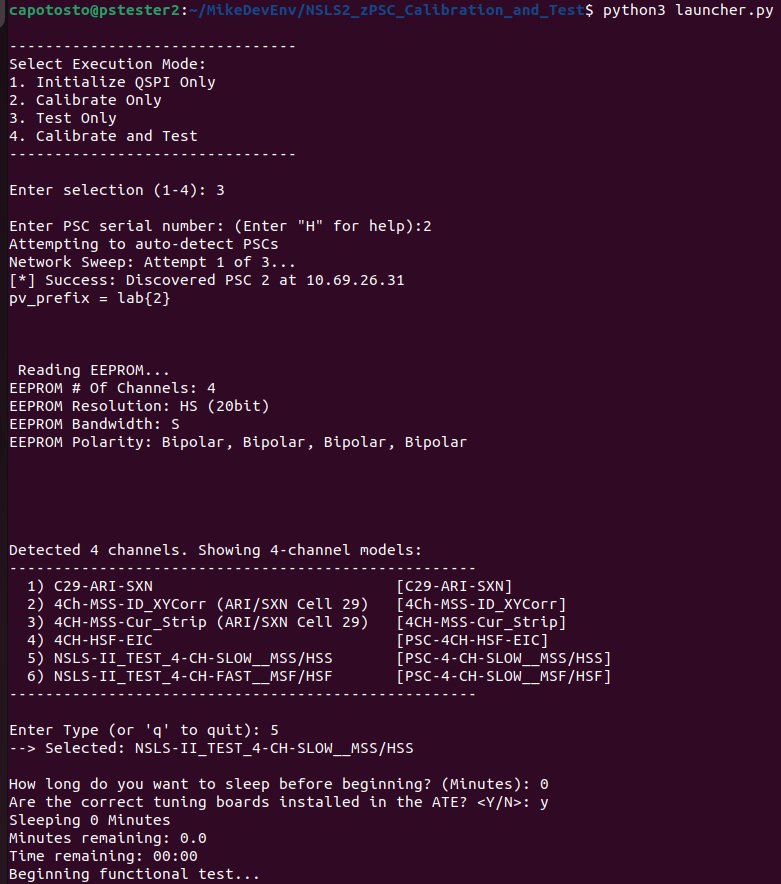
\includegraphics[width=6in]{Python_Screenshots/Test_Launch}
	\caption{Menu to launch a Test Only test of a PSC}
\end{figure}

\subsection{Option 4: Calibrate and Test}
This option will have a menu identical to that of Option 2: Calibrate Only. This simply runs the calibration script, then on completion, runs the test script. No additional figures have been included for this.


    \appendix

    % !TeX root = ../main.tex

\chapter{Example Secondary Ops Checklist}
\label{app:Example Secondary Ops Checklist}

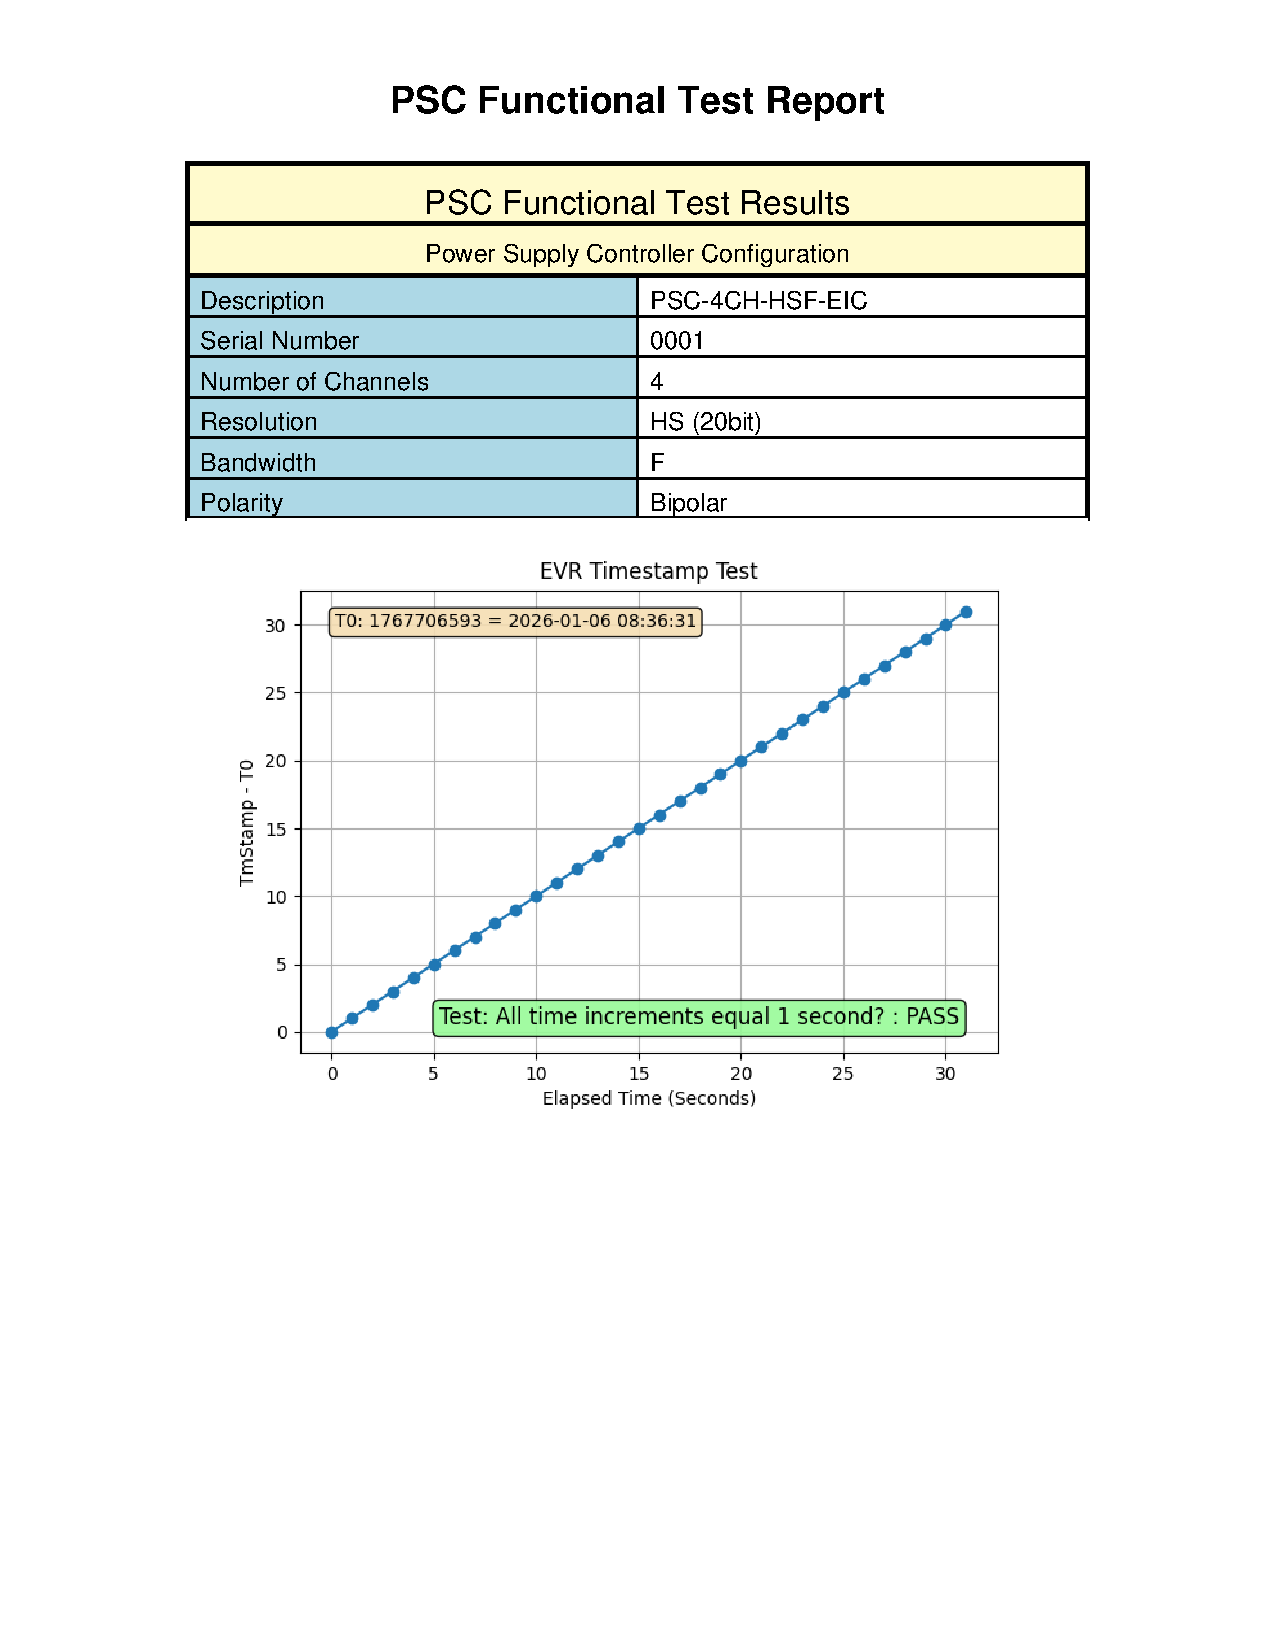
\includepdf[
pages=-,
scale=0.9,
pagecommand={}
]{./Appendices/Test_Report_Example}
    % !TeX root = ../main.tex

\chapter{Example Calibration Report}
\label{app:Example Calibration Report}

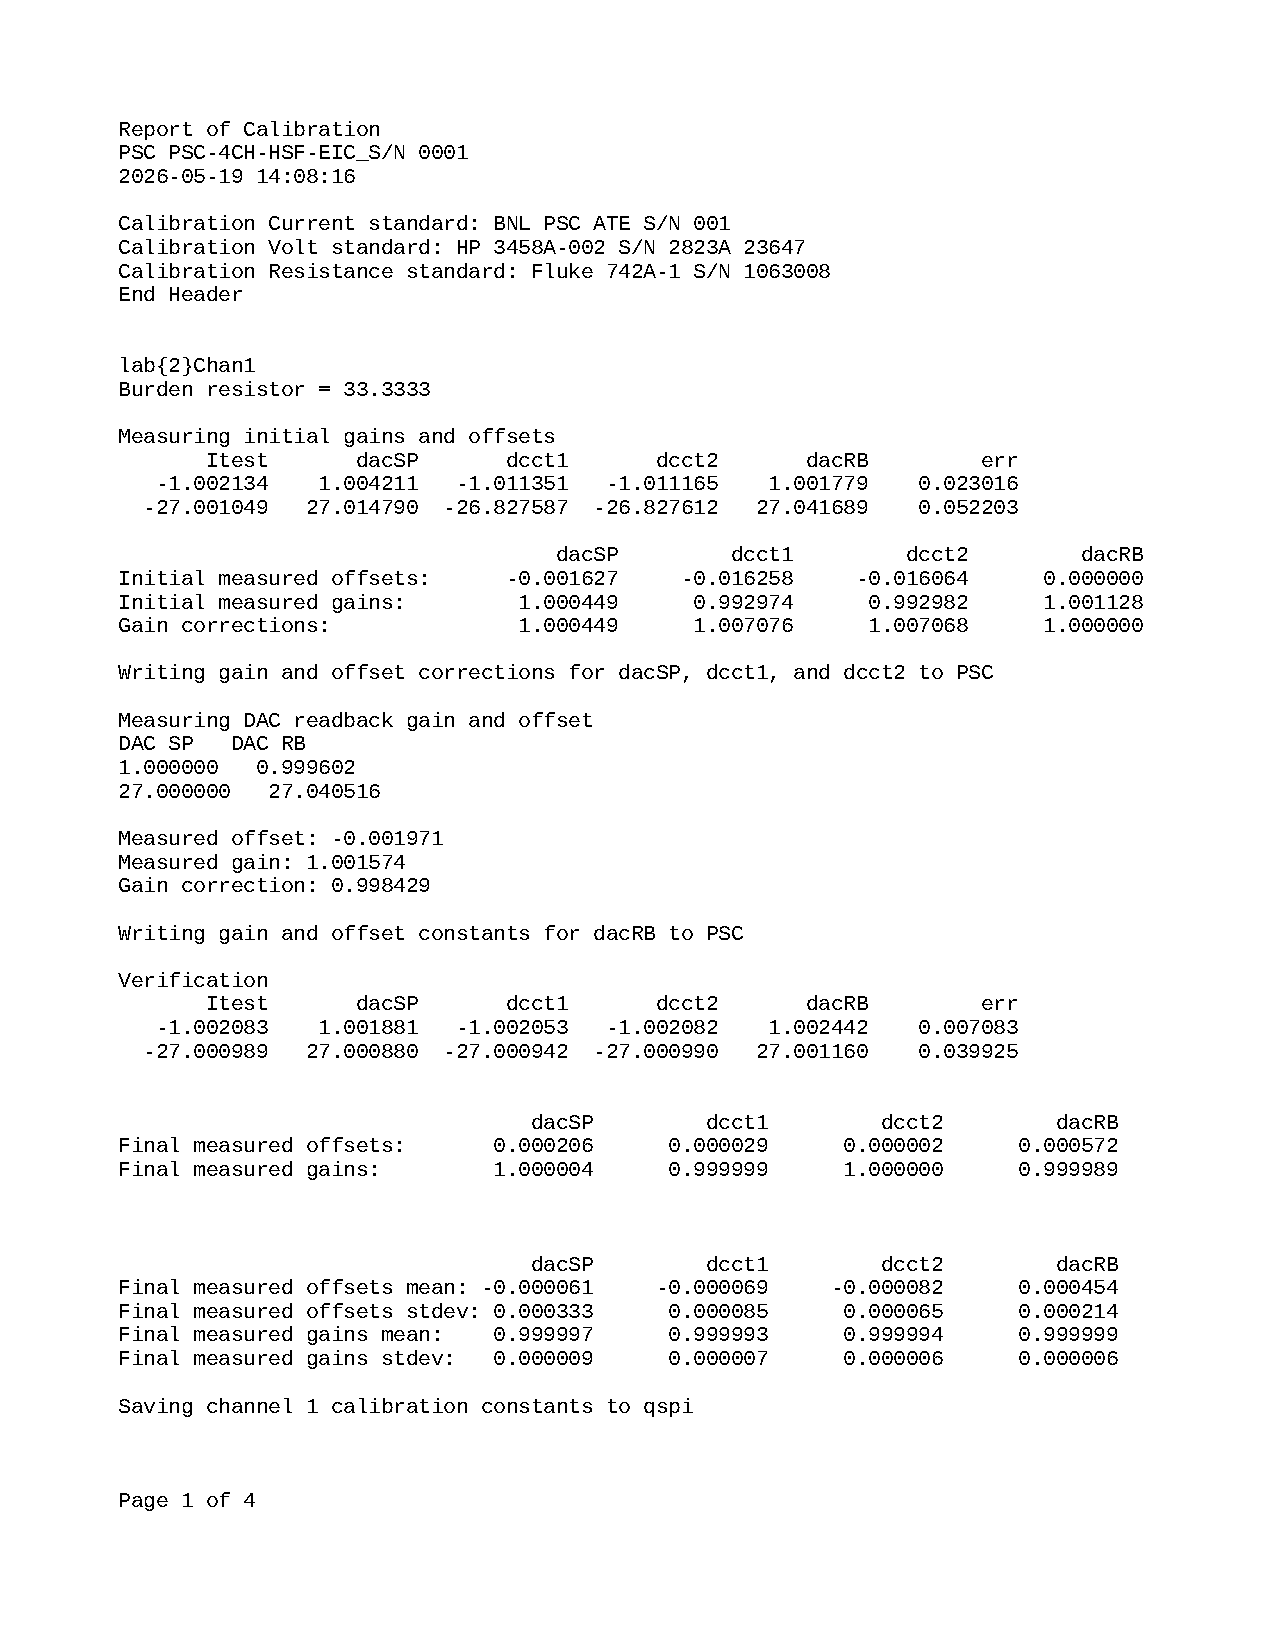
\includepdf[
pages=-,
scale=0.9,
pagecommand={}
]{./Appendices/Cal_Report_Example.pdf}
    % !TeX root = ../main.tex

\chapter{Example Test Report}

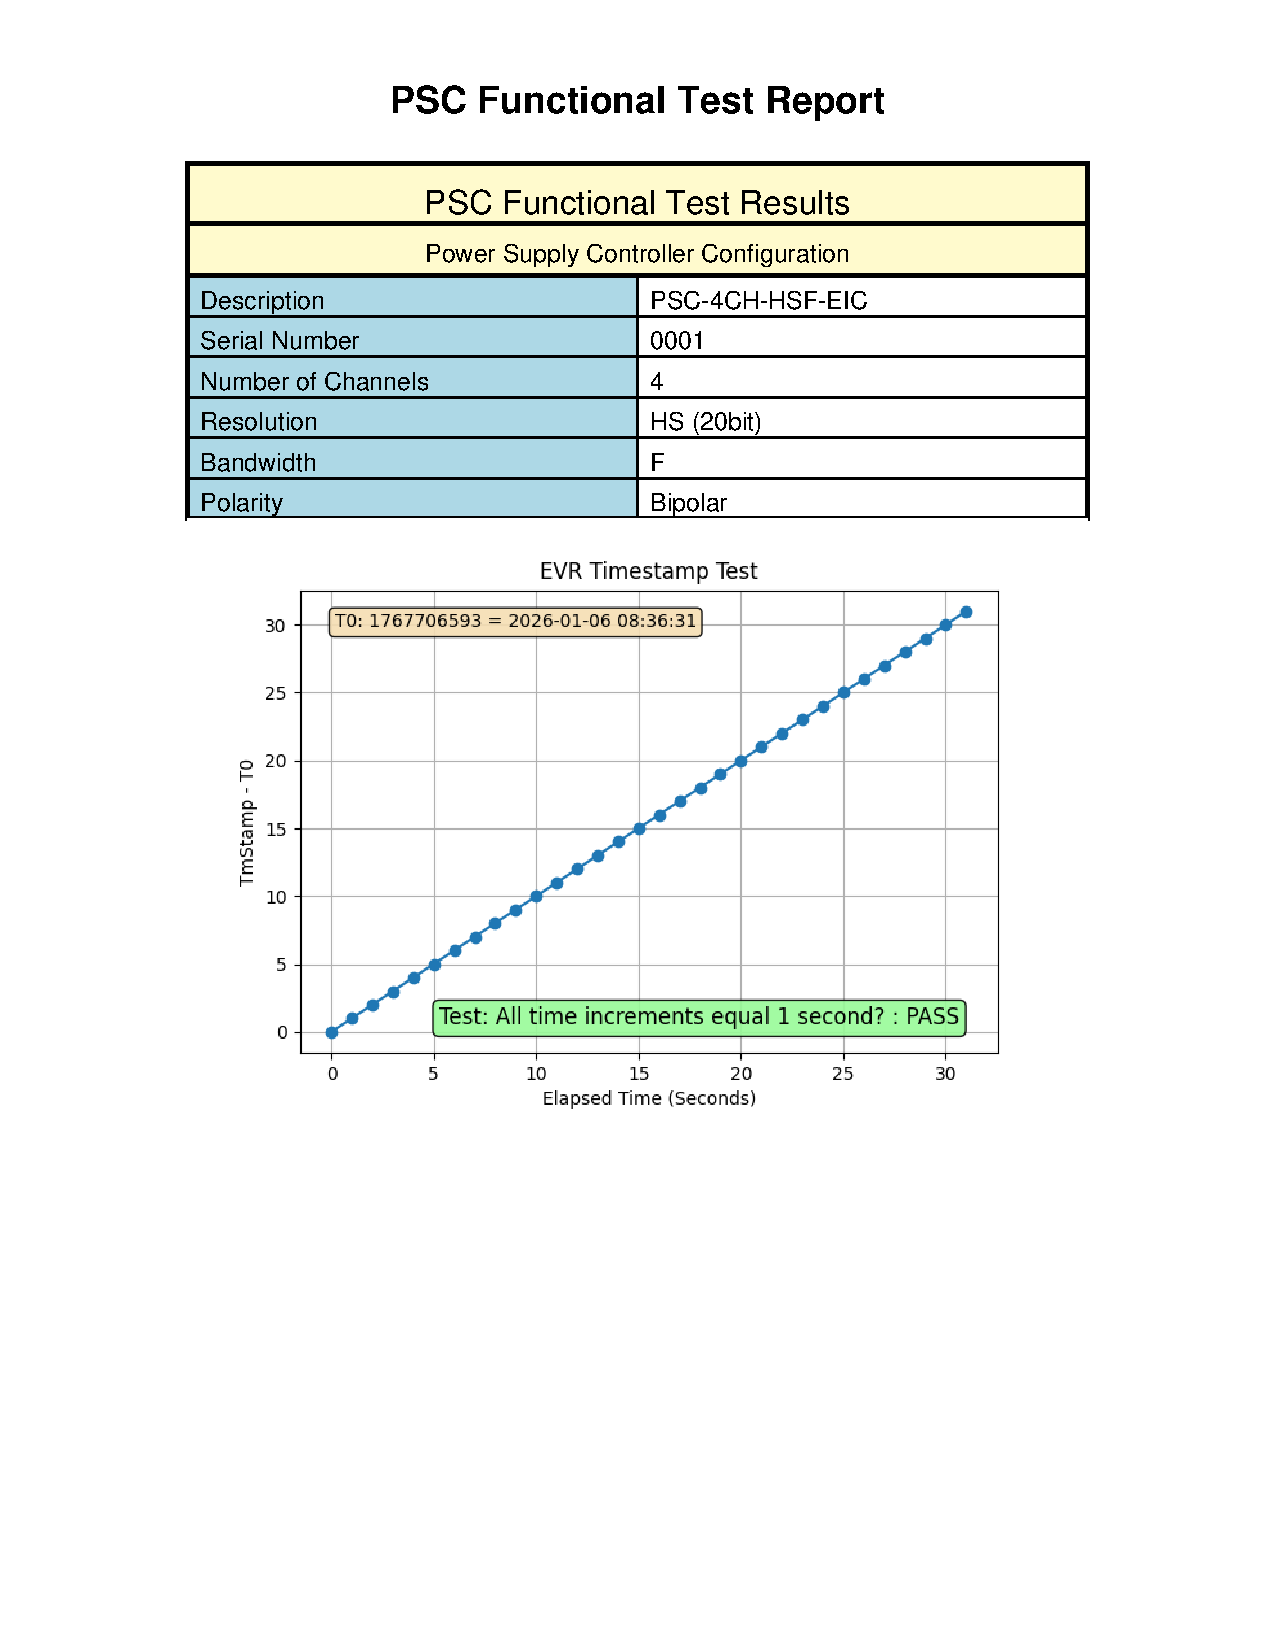
\includepdf[
pages=-,
scale=0.9,
pagecommand={}
]{./Appendices/Test_Report_Example}


    \backmatter
    % bibliography, glossary and index would go here.

\end{document}